\documentclass[10pt,twocolumn,letterpaper]{article}

\usepackage{cvpr}
\usepackage{times}
\usepackage{epsfig}
\usepackage{graphicx}
\usepackage{amsmath}
\usepackage{amssymb}
\usepackage{subcaption}
\usepackage{multirow}

% Include other packages here, before hyperref.

% If you comment hyperref and then uncomment it, you should delete
% egpaper.aux before re-running latex.  (Or just hit 'q' on the first latex
% run, let it finish, and you should be clear).
\usepackage[pagebackref=true,breaklinks=true,letterpaper=true,colorlinks,bookmarks=false]{hyperref}
\usepackage[font=small,labelfont=bf,tableposition=top]{caption}

%\cvprfinalcopy % *** Uncomment this line for the final submission

\def\cvprPaperID{****} % *** Enter the CVPR Paper ID here
\def\httilde{\mbox{\tt\raisebox{-.5ex}{\symbol{126}}}}

% Pages are numbered in submission mode, and unnumbered in camera-ready
\ifcvprfinal\pagestyle{empty}\fi
\begin{document}
%\makeatletter 
%\let\@oldmaketitle\@maketitle% Store \@maketitle
%\renewcommand{\@maketitle}
%{
%{\@oldmaketitle% Update \@maketitle to insert... 
%\centerline{
%\begin{tabular}{c}
%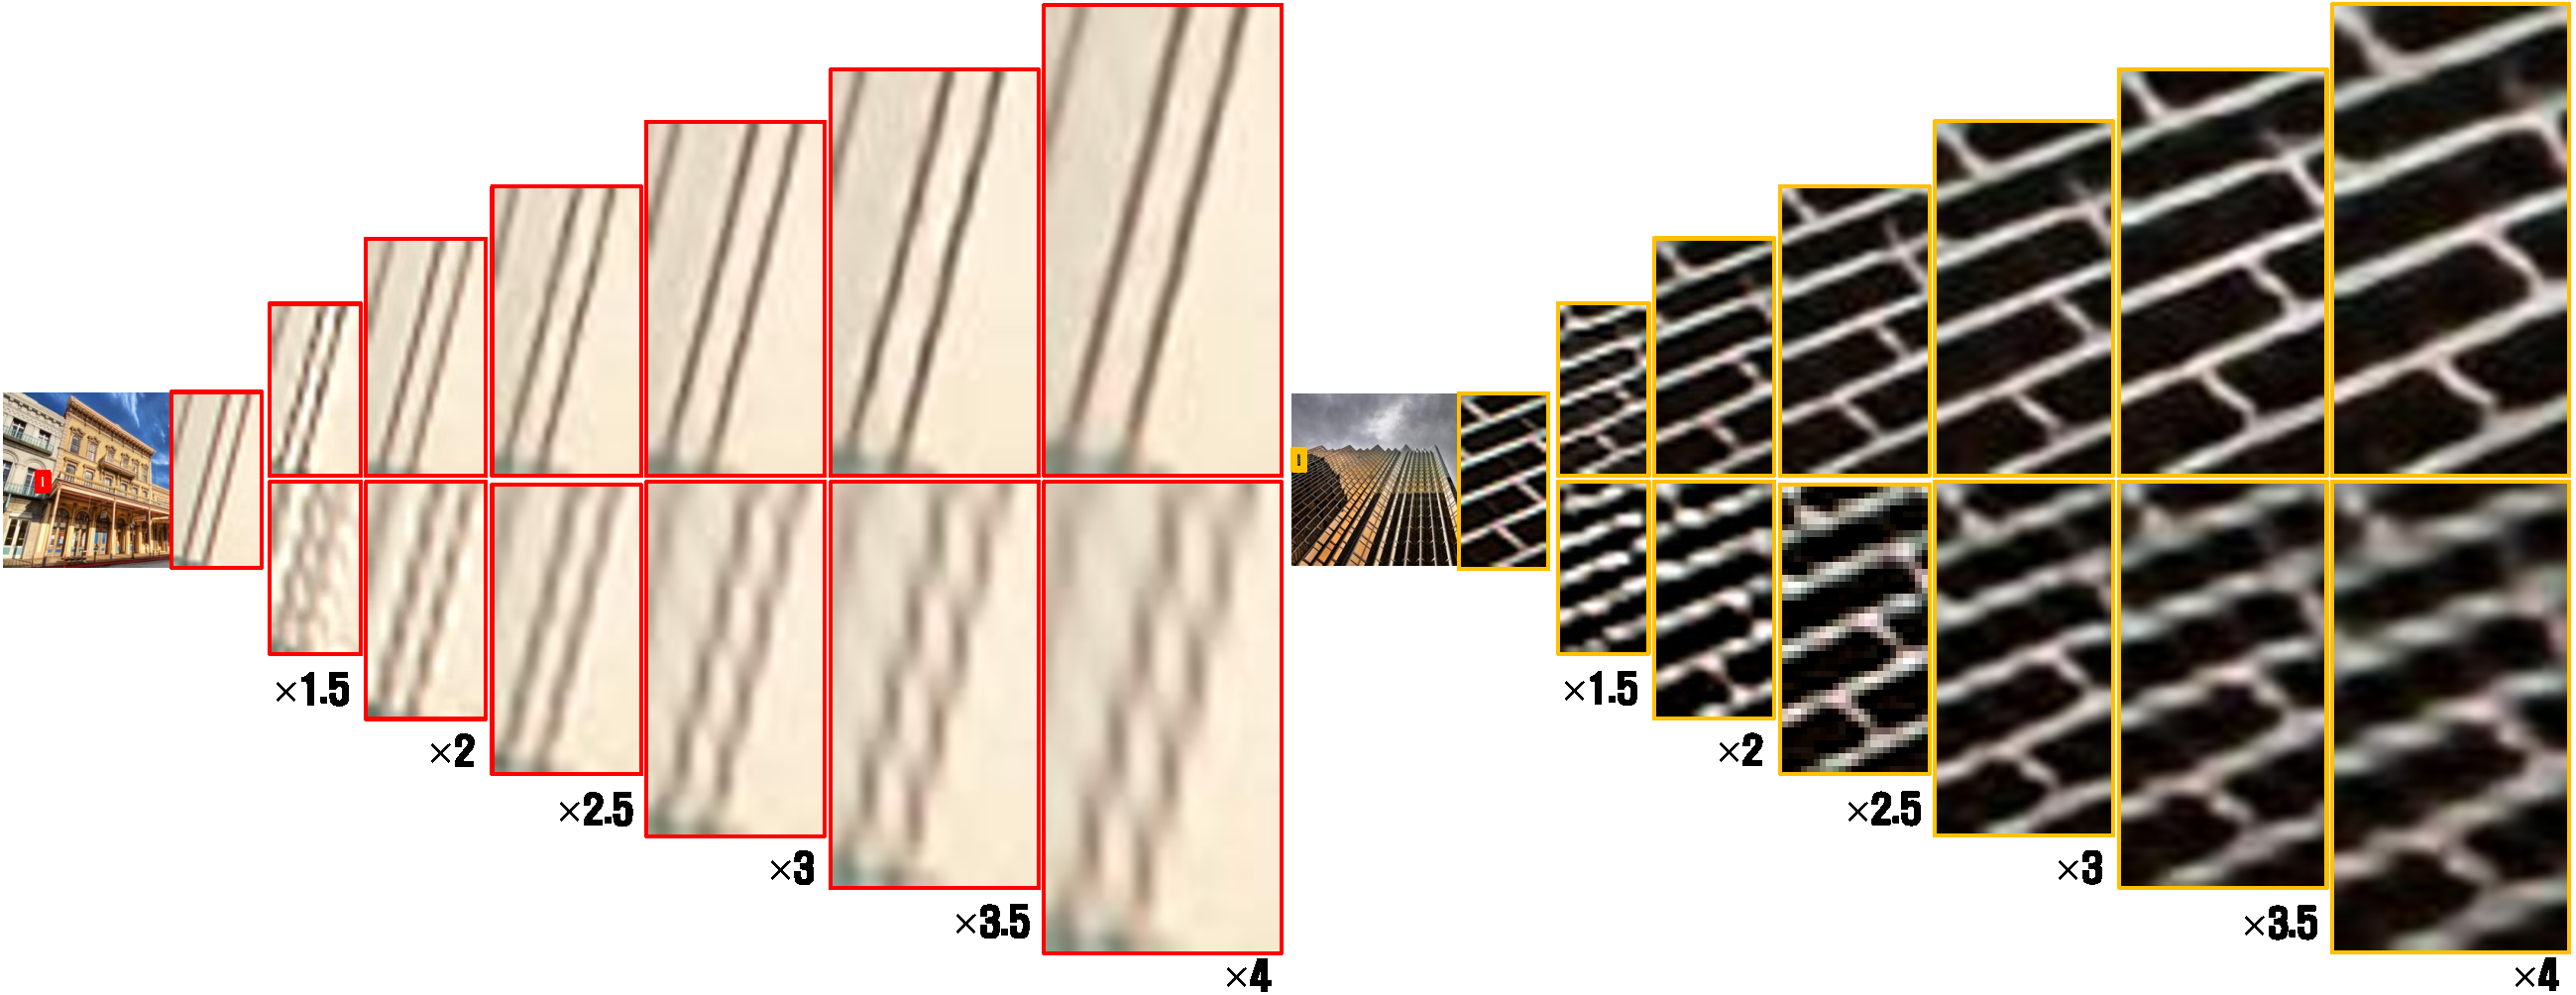
\includegraphics[width=\textwidth]{figs/fig1_sffsr.pdf}
%\end{tabular}
%%\begin{figure*}
%%\includegraphics{figs/sr10.png}
%%\end{figure*}
%}
%\bigskip}% ... an image 
%\vspace{-15pt}
%\captionof{figure}{\label{fig:fig1}
%(Top) Our results using a single network for all scale factors. Super-resolved images over all scales are clean and sharp. (Bottom)  Results of Dong et al.  \cite{Dong2014} ($\times$3 model used for all scales). Result images are not visually pleasing. To handle multiple scales, existing methods require multiple networks. }
%\vspace{15pt}
%}
%\makeatother


%%%%%%%%% TITLE
\title{Deeply-Recursive Convolutional Network for Image Super-Resolution}

\author{First Author\\
	Institution1\\
	Institution1 address\\
	{\tt\small firstauthor@i1.org}
	% For a paper whose authors are all at the same institution,
	% omit the following lines up until the closing ``}''.
	% Additional authors and addresses can be added with ``\and'',
	% just like the second author.
	% To save space, use either the email address or home page, not both
	\and
	Second Author\\
	Institution2\\
	First line of institution2 address\\
	{\tt\small secondauthor@i2.org}
}

\maketitle
%\thispagestyle{empty}




%%%%%%%%% ABSTRACT
\begin{abstract}
We propose an image super-resolution method (SR) using a deeply-recursive convolutional network (DRCN). DRCN super-resolves images with a single recursive layer. Our network utilizes very large context without dimensionality reduction such as pooling. As our method reuse the same parameters all times, our network is much smaller than the CNN-based approach with the same receptive field. As optimizing DRCN with standard gradient descent does not easily converge, we propose an SR-specific optimization method using residual-learning and (TODO change term) deep-supervision. We sucessfully learned a SR method with deep recursions (50 times). Our proposed method outperform state-of-the-art methods by a large margin (TODO:number).
%
%\pagebreak
% image super-resolution 
%While very deep CNNs, achieving outstading performances in computer vision tasks in
%We propose a recursive-convolutional network for single-image super-resolution. We  to widen 
%
%Using very deep CNNs for image super-resolution entails
%CNN-based image super-resolution requires more parameters 
%Image super-resolution requires very deep CNNs 
%As very deep CNNs (DCNN) have shown great successes in many computer vision tasks, it is natural to use one for image super-resolution. But two problems emerge: DCNN requires many parameters and 
%
%address three challenging issues of a single-image super-resolution system (SR) based on convolutional networks, which are the scale, convergence and context problems.  \textcolor{red}{Then we propose a new powerful system based on a deep residual-learning convolutional network (RCN).} 
%Scale is a serious problem of most conventional SR algorithms which can only up-sample images to a specific trained scale. In order to cope with arbitrary scales including even fractional ones, many different systems must be trained and stored for all possible scales, which is, however, practically intractable. To solve this problem, \textcolor{red}{we propose to use a single network to handle multi-scales.} The network is trained with data augmented by various scales and found to be very effective in handling multiple scales. Convergence is another critical issue in training a CNN for SR and we estimate the residual images instead of high-resolution images directly. As residuals are sparse, we find RCN converges much faster with better accuracy during training. Embedding sufficient context information \textcolor{red}{and nonlinearities} is also necessary to deal with large scale super-resolution. In our system, by cascading small filters many times in a deep network structure, contextual information over large image regions is successfully exploited. 
\end{abstract}

%%%%%%%%% BODY TEXT
\section{Introduction}
Deep convolutional networks (DCN) succeeding in various computer vision tasks typically use very large receptive fields  (224x224 is common in ImageNet classification TODO cite). Receptive field is typically enlarged by either a convolution (conv.) or a pooling (pool.).  Both approaches have drawbacks: a conv. layer introduces more parameters and a pool. layer discards some pixel-wise information. 

%While recent studies have shown that unpooling recovers some information about the original image (CITE), Alexey paper has shown inverting CNN cannot reconstruct the image perfectly.

For the task of image super-resolution (SR), receptive field corresponds to the amount of contextual information that can be exploited to infer missing high-frequency components. For example, if there exist a pattern with smoothed edges contained in a receptive field, it is plausible the pattern is recognized and edges are sharpened. As SR is an ill-posed inverse problem, collecting and analyzing more neighbor pixels can possibly give more clues on what have been lost by downsampling in which we experimentally confirm later.  

Image details are important for image restoration problems such as super-resolution and denoising. Therefore, most deep-learning approaches for such problems do not use pooling. This implies enlarging receptive field can only be achieved by introducing a new conv. layer.

Increasing depth basically introduces more parameters. Two problems can arise. First, overfitting is highly likely. More data are required for prevention. Second, model becomes too huge to be stored and retrieved (reaching gigabytes if 50 layers used TODO confirm numbers).

 
%[TODO List some efforts put into enlarging patch sizes in traditional SR literature in this paragraph.]

%[TODO Mention deep-learning SR methods.] A famous deep-learning SR method SRCNN \cite{Dong2014}, however, use only three layers resulting in a receptive field of 13 by 13. To utilize contextual information spread over very large image regions, many conv. layers need to be stacked in standard CNN settings. If $3 \times 3$ filters are stacked, stacking 10 layers result in $21 \times 21$ receptive field. This is still very small compared to typical image sizes.


To resolve the issues, we propose a SR method using a deeply-recursive convolutional network (DRCN). DRCN repeatedly applies the same convolutional layer as many times as desired. The number of parameters are kept small while widening receptive fields. Our receptive field reaches 101 by 101 and this is very large compared to patch sizes used in previous methods. 

Overfitting is largely alleviated in DRCN. As the same parameters are used again and again, the network is effectively regularized. Moreoever, our compact model can be economically stored and distributed online.   

While DRCN has good properties, learning long-range dependencies between pixels is very difficult. Networks do not easily converge. This is due to exploding/vanishing gradients. 

We propose two domain-specific approaches to ease the difficulty of training. First, residual images are modeled. Low-resolution image (input) and high-resolution image (output) share the same information to a large extent. Exact copy of Input, however, is likely to be lost during many forward passes. We explicitly add input to the final reconstruction layer. This is particularly effective when input and output are highly correlated. 


% and this phenomena is also observed in recurrent neural networks \cite{pascanu2013difficulty}. Note the difference that our recursive layer do not have any external input/output whereas recurrent neural networks have external input/output for all timesteps. 
%
%Many researchers have tackled the difficulties of training recurrent neural networks. [TODO LSTMs and GRUs and more]
%
%One way to resolve the issues is to modify our network so that memory and forget cells as in LSTM are added or gated recurrent units in GRUs are added. This severely complicates the network structure and finding the best structure involves huge efforts (TODO cite odyssey paper). 

Second, all recursions are supervised in the same manner with the same reconstruction network for all levels. This is different from deeply-supervised nets (TODO cite). In deeply-supervised net, layers have different representations across levels of abstraction (edges/parts/objects) and they are supervised in a different manner. With deep-supervision as well as residual-learning we find DRCN converges very well during training. 

%
%While SRCNN successfully introduced a deep learning technique into the super-resolution (SR) problem, it is shallow in comparison to very recent networks  (four? TODO confirm TODO cite deep net). As witenssed in several computer vision tasks, very deep networks can deliver outstanding performance. We also find that deeper SRCNN delivers better performance. 
%
%Free parameters, a weight matrix, are assigned to each layer and the number of parameters roughly correspond to the depth of a network. Deep networks, therefore, are very complex models with hugh capacities. With more parameters, overfitting is more likely unless dataset gets larger. In addition, storing huge model is not practically economical. And worse, increasing depth is often impossible due to memory limit during training. 
%
%In this work. we propose a new super-resolution method based on a recursive-convolutional network. Recursive-convolutional network was first introduced in \cite{Eigen2014}.  They did blah blah. In contrast, we do blah blah. 

\textbf{Contributions} In summary, we propose a image super-resolution method deeply recursive in nature. It utilizes very large context compared to previous SR methods with only a single convolutional layer. We suggest two ways to make this deeply-recursive convolutional network converge very fast during training: residual-learning and deep-supervision. Our algorithm demonstrates the state-of-the-art quality in common benchmarks for SR.


%Learning a mapping between low/high-resolution (LR/HR) images
%Many single image super-resolution (SR) methods are based on learning a mapping
%Transferring among scale factors???
%Writing direction: show data augmentation works for some methods.
%show limitation of SRCNN and possibly other methods.
%needs bigger depth for higher scale factors. big depth can be handled by residual-learning, faster convergence and blah.

%
%\textbf{Scale Factor} We propose a single-model SR approach. Scales are typically user-specified and can be arbitrary including fractions. For example, one might need smooth zoom-in in an image viewer or resizing to a specific dimension. Training and storing many scale-dependent models in preparation for all possible scenarios is impractical. We find a single convolutional network is sufficient for multi-scale-factor super-resolution.
%
%\textbf{Convergence} We suggest a way to speed-up the training: residual-learning CNN. As LR image and HR image share the same information to a large extent, explicitly modelling the residual image which is the difference between HR and LR images is advantageous. We propose a network structure for efficient learning when input and output are highly correlated.
%
%\textbf{Context} We utilize contextual information spread over very large image regions. For a large scale factor, it is often the case that information contained in a small patch is not sufficient for detail recovery (ill-posed). Our very deep network using large receptive field is aware of large context necessary for large-scale super-resolution.
%
%\begin{figure*}[t]
%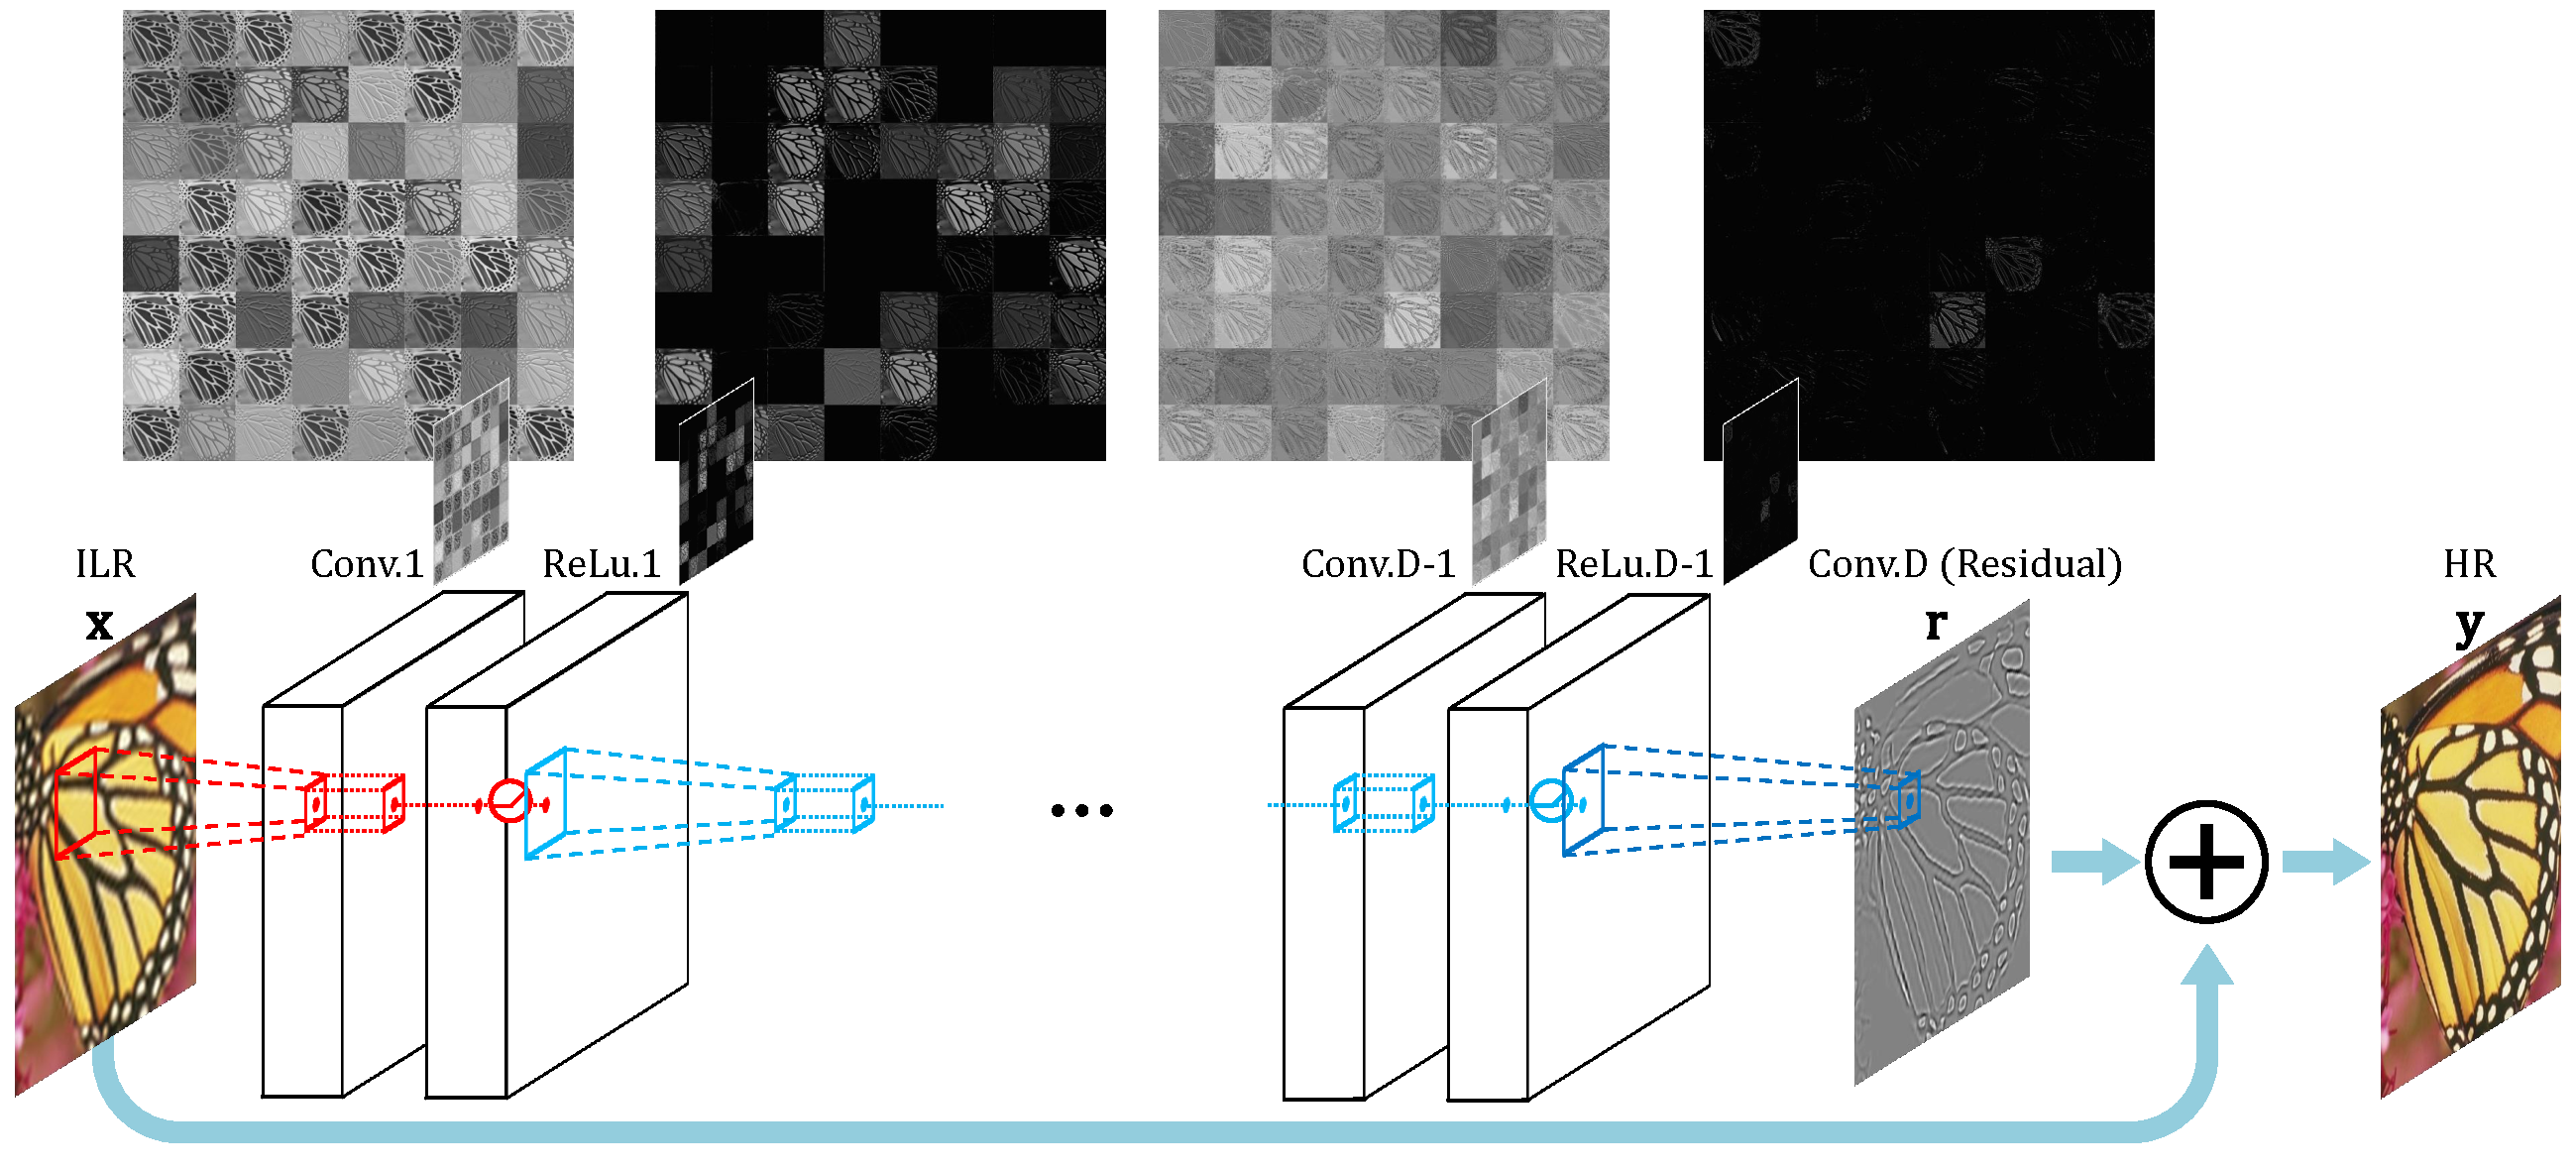
\includegraphics[width=\textwidth]{figs/fig2_sffsr.pdf}
%\caption{Our Network Structure. We cascade a pair of layers (convolutional and nonlinear) repeatedly. An interpolated low-resolution image (ILR) go through layers and transforms into a high-resolution image (HR). The network predicts a residual image and addition of ILR and residual gives the desired output. We use 64 filters for each convolutional layer and some sample feature maps are drawn for visualization. Most features after applying rectified linear units (ReLu) are zero.}
%\label{fig:network}
%\end{figure*}


\section{Related Work}
\subsection{Single-Image Super-Resolution}

We address the problem of generating a high-resolution (HR) image given a low-resolution (LR) image, commonly referred as single image super-resolution (SISR) \cite{Irani1991}, \cite{freeman2000learning}, \cite{glasner2009super}. SISR is widely used in computer vision applications ranging from security and surveillance imaging to medical imaging where more image details are required on demand.

Many SISR methods have been studied in the computer vision community. Interpolation methods are simple and very fast but they give poor results. More powerful methods utilize statistical image priors \cite{sun2008image,Kim2010} or rely on internal patch recurrence \cite{glasner2009super, Huang-CVPR-2015}.

Recently, sophisticated learning methods are widely used to model a mapping from LR to HR patches. Existing methods use various techniques: neighbor embedding \cite{chang2004super,bevilacqua2012}, sparse coding \cite{yang2010image,zeyde2012single,Timofte2013,Timofte}, convolutional neural network (CNN) \cite{Dong2014} and random forest \cite{schulter2015fast}.

While many methods focus on how regression functions from LR to HR are modeled, not much attention has paid to long-range dependencies among pixels. This is closely related to patch sizes and receptive fields used in their methods. In Section (TODO), we discuss pixel interaction in detail.


%[JL TODO] Discuss patch sizes of previous methods.

%Among them, Dong et al. \cite{Dong2014} has demonstrated that a CNN can be used to learn a mapping from LR to HR in an end-to-end manner. Their method, termed SRCNN, does not require any engineered features that are typically necessary in other methods \cite{yang2010image,zeyde2012single,Timofte2013,Timofte}. In addition, it is very fast and accurate.

%\subsection{Convolutional Network  for Image Restoration}
%
%We address the problem of generating a high-resolution (HR) image given a low-resolution (LR) image, commonly referred as single image super-resolution (SISR) \cite{Irani1991}, \cite{freeman2000learning}, \cite{glasner2009super}. SISR is widely used in computer vision applications ranging from security and surveillance imaging to medical imaging where more image details are required on demand.
%
%Many SISR methods have been studied in the computer vision community. Interpolation methods such as bicubic interpolation and Lanczos resampling \cite{duchon1979lanczos} are simple and very fast but they give poor results. More powerful methods utilize statistical image priors \cite{sun2008image,Kim2010} or rely on internal patch recurrence \cite{glasner2009super}.
%
%Recently, sophisticated learning methods are widely used to model a mapping from LR to HR patches. Existing methods use various techniques: neighbor embedding \cite{chang2004super,bevilacqua2012}, sparse coding \cite{yang2010image,zeyde2012single,Timofte2013,Timofte} and convolutional neural network (CNN) \cite{Dong2014}.
%
%Among them, Dong et al. \cite{Dong2014} has demonstrated that a CNN can be used to learn a mapping from LR to HR in an end-to-end manner. Their method, termed SRCNN, does not require any engineered features that are typically necessary in other methods \cite{yang2010image,zeyde2012single,Timofte2013,Timofte}. In addition, it is very fast and accurate.
%
\subsection{Recursive Neural Network in Computer Vision}

%
%Recursive convolution is first proposed in \cite{Eigen2014}. (Socher et al. [45]?? Eigen et. al) to understand deep architectures. They used up to three 

Recursive neural networks, suitable for temporal and sequential data, have seen limited use on algorithms operating on a single static image.   Socher et al.  \cite{socher2012convolutional} used a convolutional network in a separate stage to first learn features on RGB-Depth data, prior to hierarchical merging. In these models the input dimension is twice that of the output and recursive convolutions are applied only two times. In Eigen et. al \cite{Eigen2014}, recursive layers have the same input and output dimension, but recursive convolutions resulted in worse performances than a single convolution due to overfitting. 

To overcome overfitting, Liang and Hu \cite{Liang_2015_CVPR} uses a recurrent layer that takes feed-forward inputs into all unfolded layers. They show that up to three convolutions performance increases. Their network is for object recognition and the architecture is vastly similar to existing architectures, except each convolution is applied three times. 

While \cite{Eigen2014} and \cite{Liang_2015_CVPR} simply modify existing architectures to apply convolutions up to three times, our network is completely different from multi-layer approaches. To our knowledge, we demonstrate for the first time that a single recursive layer can entirely solve a non-trivial vision task (SR). 

In addition, we demonstrate that recursions can be very deep. We apply the same convolution up to TODO 30 times (previous maximum is three). It is an interesting future direction to see if a single-layer approach works for other tasks.  

%
%\subsection{Convolutional Network for Image Super-Resolution}
%Recently, Dong et al. \cite{Dong2014} have presented a SISR method called SRCNN using a convolutional network. Let us first analyze SRCNN in three aspects: scale, convergence and context.
%
%\textbf{Scale} SRCNN is trained for a single scale factor and supposed to work only with the specified scale. Given a user-specified scale, the corresponding network is retrieved for the task. If new scale is on demand, new model has to be trained. Most existing methods including not only SRCNN but also other regression-based methods \cite{Timofte2013, Timofte, Yang2013} are in this paradigm. So, in these frameworks, the general super-resolution task is decomposed into multiple sub-tasks, where each sub-task is a single-scale super-resolution. Each sub-task is solved by a super-resolution machine, trained to be an expert for the corresponding scale. 
%
%However, preparing many individual machines for all possible scenarios to cope with multiple scales is inefficient since many systems with the same structure need to be trained and stored.
%We attempt to reinterpret the task in our work and try to use a single machine to solve all sub-tasks, multi-scale. This turns out to work very well. Our single machine is compared favorably to a single-scale expert for the given sub-task. \textcolor{red}{In addition, scale augmentation actually enriches training data and utilizes the capacity of deep networks.} 
%
%\textbf{Convergence}
%For training, SRCNN directly model high-resolution images so that the convergence rate is very slow. In contrast, our network models the residual images, i.e., the image details. We find convolution network converge much faster with better accuracy during training.
%
%\textbf{Context}
%SRCNN consists of only three layers: patch extraction/representation, non-linear mapping and reconstruction. They use filters with spatial sizes $9\times9$, $1\times1$, $5\times5$, respectively. Number of filters are 64, 32 and 1, where the last layer corresponds to the output (gray-scale image). In more recent work by Dong et al. \cite{dong2014image}, they conclude that deeper networks do not result in better performance.
%
%In contrast, we use 20 layers of the same type (64 filters of size $3\times3$ for each layer) except the last layer for image reconstruction. Our network is very deep (20 vs. 3) and information used for reconstruction (receptive field) is much larger ($41\times41$ vs. $13\times13$).
%
%\textcolor{red}{With above improvements,} our network delivers better performance than SRCNN. In addition, our output image has the same size as the input image by padding zeros every layer during training whereas no padding is used in training SRCNN. Finally, we use the same learning rates for all layers while SRCNN uses different learning rates for different layers.
%
%
%\begin{table*}[t]
%	\small
%	\centering
%\begin{tabular}
%{|c|c|c|c|c|c|c|c||c|}
%\hline 
% Test / Train & {$\times$2}& {$\times$3}& { $\times$4}& {$\times$2,3}& {$\times$2,4}& { $\times$3,4}& {$\times$2,3,4} & {Bicubic} \\
%\hline
%$\times$2  & \color{red} 37.10  & 30.05  & 28.13  & \color{red} 37.09  & \color{red} 37.03  & 32.43  & \color{red}37.06 &33.66   \\
%$\times$3  & 30.42  & \color{red} 32.89  & 30.50  & \color{red} 33.22  & 31.20  & \color{red} 33.24  & \color{red} 33.27  & 30.39 \\
%$\times$4  & 28.43  & 28.73  & \color{red} 30.84  & 28.70  & \color{red} 30.86  & \color{red} 30.94  & \color{red} 30.95 & 28.42  \\
%\hline
%\end{tabular}
%	\vspace{1pt}
%	\caption{Scale Factor Experiment. Several models are trained with different scale sets. Quantitative evaluation (PSNR) on dataset `Set5' is provided for scale factors 2,3 and 4.  {\color{red}Red color} indicates test scale is included during training. Models trained with multiple scales perform well on the trained scales. }
%	\label{tab:SRCNN_Factor_Test}
%\end{table*}
%
\section{Proposed Method}
In this section, our proposed method is explained. We first go over the process of super-resolving an image with our recursive-convolutional network (inference). Next, we describe the training procedure.

\subsection{Inference}
  \begin{align*}
        H_0 &= max(0, W_{xh_0}*X + b_{h_{0})}\\
        H_1 &= max(0, W_{h_0 h_1}*H_0 + b_{h_{1})}\\
        H_d &= max(0, W_{hh}*H_{d-1} + b_h), d = 2, ..., D - 1\\
        H_D &= max(0, W_{h h_D}*H_{D-1} + b_{h_D})\\
        \hat{Y} &= max(0, W_{hy}*H_{D} + b_y)
    \end{align*}

%\subsubsection{Convolutional Network}
%Simonyan and Zisserman \cite{simonyan2015very} have demonstrated the effectiveness of stacking small filters ($3\times3$) many times to make the network (very) deep (VGG-net). Inspired by VGG-net, we stack small filters repeatedly. We first describe our deep convolutional network (DCN) and then explain how to make it recursive.
%
%The DCN configuration is outlined in Figure \ref{fig:network}. We use $d$ layers where layers except the first and the last are of the same type: $F$ filters of the size $3\times 3 \times F$, where a filter operates on $3\times3$ spatial region across $F$ channels (feature maps). The first layer operates on the input image. The last layer, used for image reconstruction, consists of a single filter of size $3\times 3 \times F$.
%
%The network takes an interpolated input image (to the desired size) as input and predicts image details. While modelling image details is often used in super-resolution methods \cite{Timofte2013, Timofte, bevilacqua2012,bevilacqua2013super}, to our knowledge, there has been no CNN-based method that models image details explicitly.
%
%In this work, we demonstrate explicitly modelling image details is sufficient for the purpose of SR and has several advantages. These are further justified and discussed later in the Section \ref{sec:residual}. 
%
%One problem with applying a deep network to predict dense outputs is that the size of feature map gets reduced every time convolution operations are applied. For example,  when an input of size $(n+1)\times (n+1)$ is applied to a network with receptive field size $n\times n$, the output image is $1\times1$. 
%
%This is in accordance with other super-resolution methods since many require surrounding pixels to infer center pixels correctly. This center-surround relation is useful since surrounding region provides more constraints to this ill-posed problem (SR). For pixels near image boundary, this relation cannot be exploited to the full extent and many SR methods crop the result image. 
%
%This methodology, however, is not valid if required surround region is very big. After cropping, the final image is too small to be visually pleasing.
%
%To resolve this issue, we opt not to use this relation. Instead, we use the same-sized regions (i.e. $n\times n$ input and output). To do this, we pad zeros before convolutions to keep the sizes of all feature maps (including the output image) the same. We think that powerful nonlinearities modelled by CNNs can handle both the general case (i.e. receptive field has all valid pixels) and the corner case (i.e. the field located near the image boundary has invalid pixels beyond the border).
%
%It turns out that zero-padding works surprisingly well. For this reason our method differs from most other methods in the sense that pixels near image boundary are also correctly predicted. 
%
%Once image details are predicted, they are added back to ILR to give the final result (HR). We use this structure for all experiments in our work.  
%
%\subsubsection{Recursive-Convolutional Network}
%
%TODO
%
%\begin{figure*}[t]
%	\centering
%	\begin{subfigure}{0.3\textwidth}
%		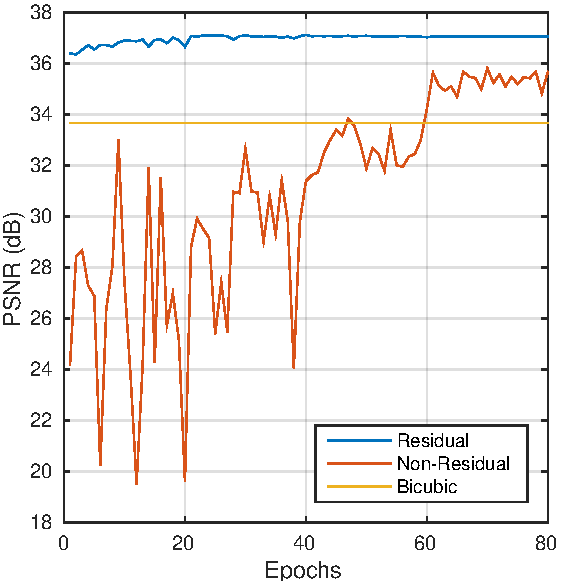
\includegraphics[width=\textwidth]{figs/residual_exp0}
%		\caption{Initial learning rate 0.1}
%		\label{fig:gull}
%	\end{subfigure}%
%	\hfill
%	%(or a blank line to force the subfigure onto a new line)
%	\begin{subfigure}{0.3\textwidth}
%		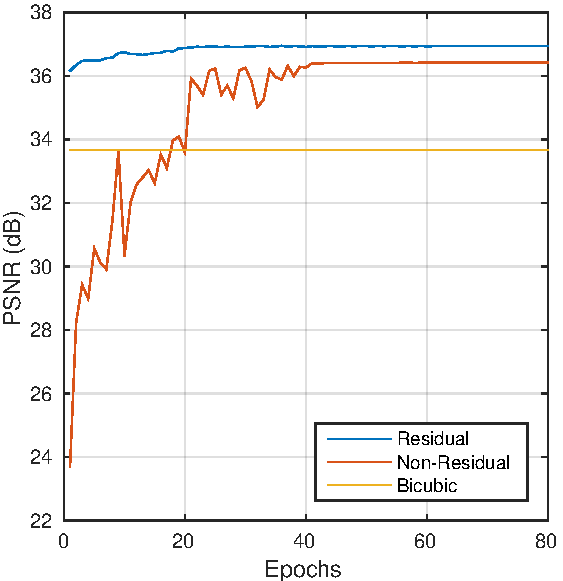
\includegraphics[width=\textwidth]{figs/residual_exp1}
%		\caption{Initial learning rate 0.01}
%		\label{fig:tiger}
%	\end{subfigure}
%	\hfill
%	\begin{subfigure}{0.3\textwidth}
%		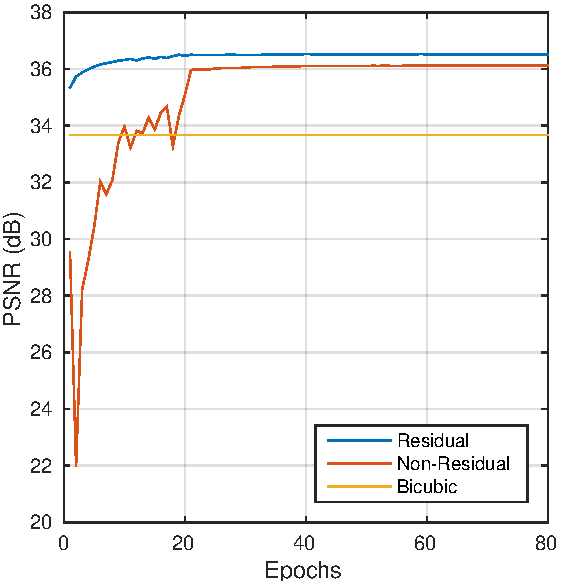
\includegraphics[width=\textwidth]{figs/residual_exp2}
%		\caption{Initial learning rate 0.001}
%		\label{fig:mouse}
%	\end{subfigure}
%	\caption{Performance curve for residual and non-residual networks. Two networks are tested under `Set5' dataset with scale factor 2. Residual networks quickly reaches state-of-the-art performance within a few epochs, whereas non-residual network (which models high-resolution image directly) takes many epochs to reach its maximum performance. Moreover, the final accuracy is higher for residual network.}
%	\label{fig:residual2}
%\end{figure*}
%
%\begin{figure*}[t]
%\vspace{-.5cm}
%	\centering
%	\begin{subfigure}{0.25\textwidth}
%		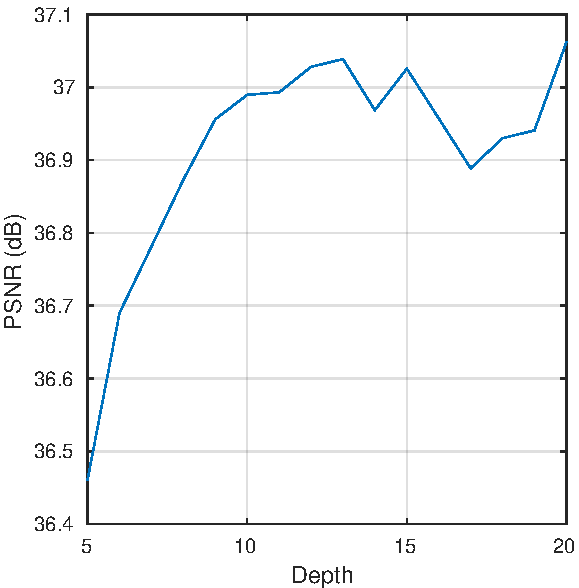
\includegraphics[width=\textwidth]{figs/depth_exp1}
%		\caption{Test Scale Factor 2}
%		\label{fig:gull}
%	\end{subfigure}%
%	\quad
%	%(or a blank line to force the subfigure onto a new line)
%	\begin{subfigure}{0.25\textwidth}
%		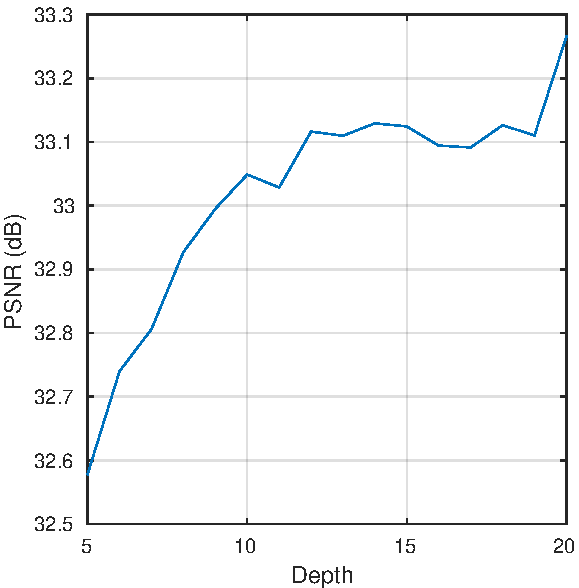
\includegraphics[width=\textwidth]{figs/depth_exp2}
%		\caption{Test Scale Factor 3}
%		\label{fig:tiger}
%	\end{subfigure}
%	\quad
%	\begin{subfigure}{0.25\textwidth}
%		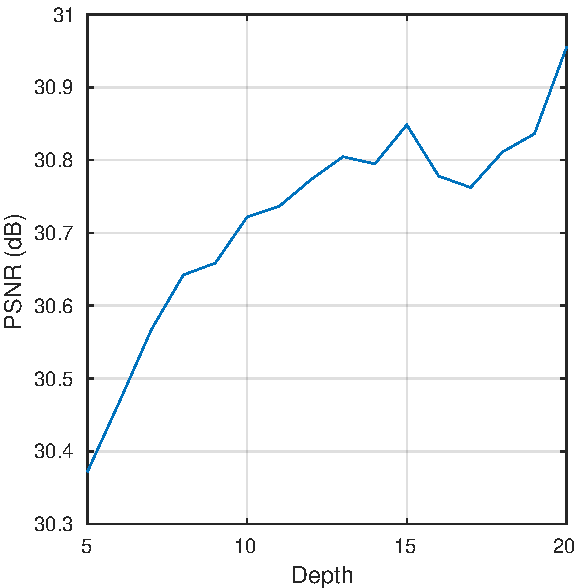
\includegraphics[width=\textwidth]{figs/depth_exp3}
%		\caption{Test Scale Factor 4}
%		\label{fig:mouse}
%	\end{subfigure}
%	\caption{Depth vs Performance}\label{fig:depth}
%\end{figure*}
%
%
%\subsection{Training}
%
%We now describe the objective to minimize to find optimal parameters of our model. Let ${\bf x}$ denote an interpolated low-resolution image and ${\bf y}$ a high-resolution image. 
%Given training dataset $\{{\bf x}^{(i)},{\bf y}^{(i)}\}{}_{i=1}^{N}$, our goal is to learn a model $f$ that predicts values $\mathbf{\hat{y}}=f(\mathbf{x})$.
%
%In the least-squares regression setting, typically used in super-resolution
%problems, the mean squared error $\frac{1}{2}||\mathbf{y}-f(\mathbf{x})||^{2}$
%averaged over training set is minimized. This favors high Peak Signal-to-Noise
%Ratio (PSNR), a widely-used evaluation criteria for SR. 
%
%As the input and output images are mostly similar, we define a residual image ${\bf r}={\bf y}-{\bf x}$, where most values are likely to be \textcolor{red}{zero or} small. We want to predict this residual image. The loss function now becomes $\frac{1}{2}||\mathbf{r}-f(\mathbf{x})||^{2}$, where $f(\bf{x})$ is the network prediction. Loss function is one major difference between SRCNN and ours. 
%
%In networks, this is reflected in the loss layer as follows. 
%Our loss layer takes three inputs: residual estimate, network input (ILR) and ground truth HR. The loss is computed as the Euclidean distance between the reconstructed image (the sum of network input and output) and ground truth. With this residual loss layer, we can still use the original dataset for an end-to-end learning.
%
%Training is carried out by optimizing the regression objective using mini-batch gradient descent based on back-propagation (LeCun et al. \cite{lecun1998gradient}). We set the momentum parameter to 0.9. The training is regularized by weight decay ($L_2$ penalty multiplied by
%0.0001).  
%
%Training deep models often fail to converge. He et al. \cite{he2015delving} uses a theoretically sound initialization method which helps very deep models converge when training from scratch and they succeed in training 30 weight layers. They, however, report no benefit from training extremely deep models for their problem. In our work, adding layers are beneficial in general. For large scale factors, deep models exploiting contextual information spread in very large field are dominant. 
%
%Training the multi-scale model is straightforward. Training datasets for several specified scales are combined into one big dataset. We demonstrate in the next section that a model learned with this works under multiple scales.  
%
%\textcolor{red}{Data preparation is similar to SRCNN \cite{Dong2014} with some differences. Input patch size is equal to the size of receptive field and images are divided into sub-images with no overlap. 64 sub-images constitue a mini-batch, where sub-images from different scales can be in the same batch.}
%
%We implement our model using the \textit{MatConvNet}\footnote{\url{ http://www.vlfeat.org/matconvnet/}} package \cite{arXiv:1412.4564}.
%
%\section{Understanding Properties}
%
%\subsection{Effectiveness of Recursion}
%In this section, we compare our recursive network to canonical CNNs.  
%
%TODO plot performance curve and parameter curves (RCN flat)
%
%In this section, we study three properties of our proposed method. First, we show our method with a single network performs as well as a method using multiple networks trained for each scale. We can effectively reduce model capacity (the number of parameters) of multi-network approaches.
%
%Second, we show our residual-learning network converges very fast in relative to the standard CNN. Moreover, our network gives a significant boost in performance. 
%
%Third, we show large depth is necessary for the task of SR. A very deep network utilizes more contextual information in an image \textcolor{red}{and models complex functions with many nonlinear layers.} We experimentally confirm that deeper networks give better performances than shallow ones. 
%
%\subsection{Single Model for Multiple Scales}
%Scale augmentation during training is a key technique to equip a network with super-resolution machines of multiple scales. Many SR processes for different scales can be executed with our multi-scale machine with much smaller capacity than that of single-scale machines combined. 
%
%We start with an interesting experiment as follows: we train our network with a scale factor $s_{\text{train}}$ and it is tested under another scale factor $s_{\text{test}}$. Here, factors 2,3 and 4 that are widely used in SR comparisons are considered. Possible pairs ($s_{\text{train}}$,$s_{\text{test}}$) are tried for the dataset `Set5' \cite{bevilacqua2012}. Experimental results are summarized in Table \ref{tab:SRCNN_Factor_Test}. 
%
%Performance is degraded if $s_{\text{train}} \neq s_{\text{test}}$. For scale factor 2, the model trained with factor 2 gives PSNR of 37.10 (in dB), whereas models trained with factor 3 and 4 give 30.05 and 28.13, respectively. A network trained over single-scale data is not capable of handling other scales. In many tests, it is even worse than bicubic interpolation, the method used for generating the input image. 
%
%We now test if a model trained with scale augmentation is capable of performing SR at multiple scale factors. The same network used above is trained with multiple scale factors $s_{\text{train}} = \{2,3,4\}$. In addition, we experiment with the cases $s_{\text{train}} = \{2,3\}, \{2,4\}, \{3,4\}$ for more comparisons. 
%
%We observe the network copes with any scale used during training. When $s_{\text{train}} = \{2,3,4\}$ ($\times 2, 3, 4$ in Table \ref{tab:SRCNN_Factor_Test}), its PSNR for each scale is comparable to those achieved from the corresponding result of single-scale network: 37.06 vs. 37.10 ($\times 2$), 33.27 vs. 32.89 ($\times 3$), 30.95 vs. 30.86 ($\times 4$).
%
%Another pattern is that for large scales ($\times 3,4$), our multi-scale network performs over single-scale network: our model ($\times 2,3$), ($\times 3,4$) and ($\times 2, 3,4$) give PSNRs 33.22, 33.24 and 33.27 for test scale 3, respectively, whereas ($\times 3$) gives 32.89. Similarly, ($\times 2,4$), ($\times 3,4$) and ($\times 2, 3,4$) give 30.86, 30.94 and 30.95 (vs. 30.84 by $\times 4$ model),  respectively. From this, we observe training multiple scales boost the performance for large scales.
%
%\subsection{Residual Images for Better Learning}
%\label{sec:residual}
%
%As we already have low-resolution image as input, predicting high-frequency components is enough for the purpose of SR. Predicting residuals (HR - ILR) is widely used in several previous methods \cite{Timofte2013, Timofte,zeyde2012single}. However, it has not been studied in the context of deep-learning-based SR.
%
%In this work, we have proposed a network structure that learns from a residual image (ground truth minus input, i.e. high-resolution image minus interpolated low-resolution). We now study the effect of this modification to a standard CNN structure in detail. 
%
%First, we find this residual network converge much faster. Two networks are compared experimentally: residual network and standard network. We use depth 10 (weight layers) and scale factor 2. Performance curves for various learning rates are shown in Figure \ref{fig:residual2}. All use the same learning rate scheduling mechanism that has been mentioned above. 
%
%Second, at convergence, the residual network shows superior performance. In \textcolor{red}{Figure \ref{fig:residual2}}, residual networks give higher PSNR when training is done. 
%
%In short, this simple modification to a standard network structure is beneficial and one can explore the validity of the idea in other image restoration problems. 
%
%\begin{figure}
%\vspace{-1cm}
%\centering
%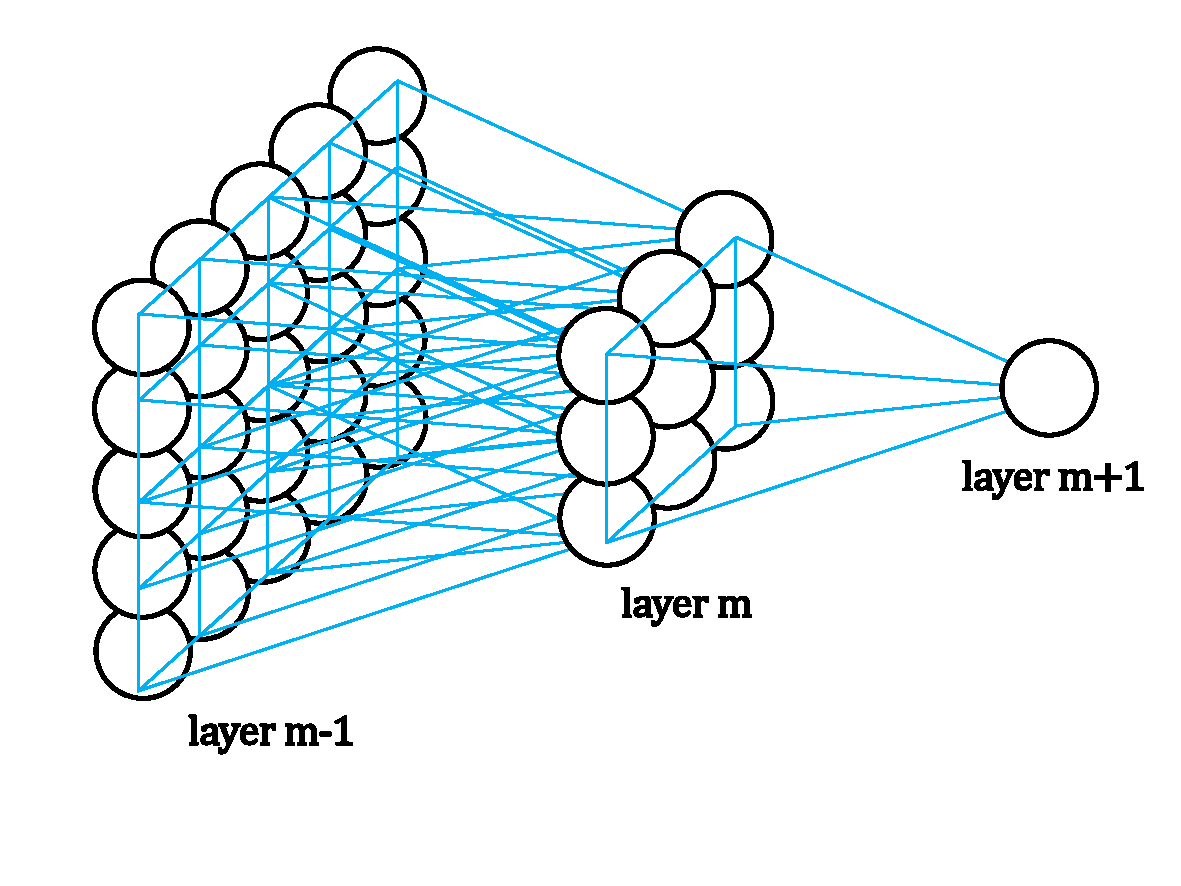
\includegraphics[scale=0.3]{figs/fig4_sffsr.pdf}
%\vspace{-0.7cm}
%\caption{Receptive field for a neuron in network grows as layers are stacked. In our work, up to 20 layers are used reaching 41$\times$41 at maximum. }
%\label{fig:receptive_field}
%\end{figure}
%
%
%\begin{figure*}
%\begin{center}
%\begin{tabular}{ccccc}
%\graphicspath{{figs/}}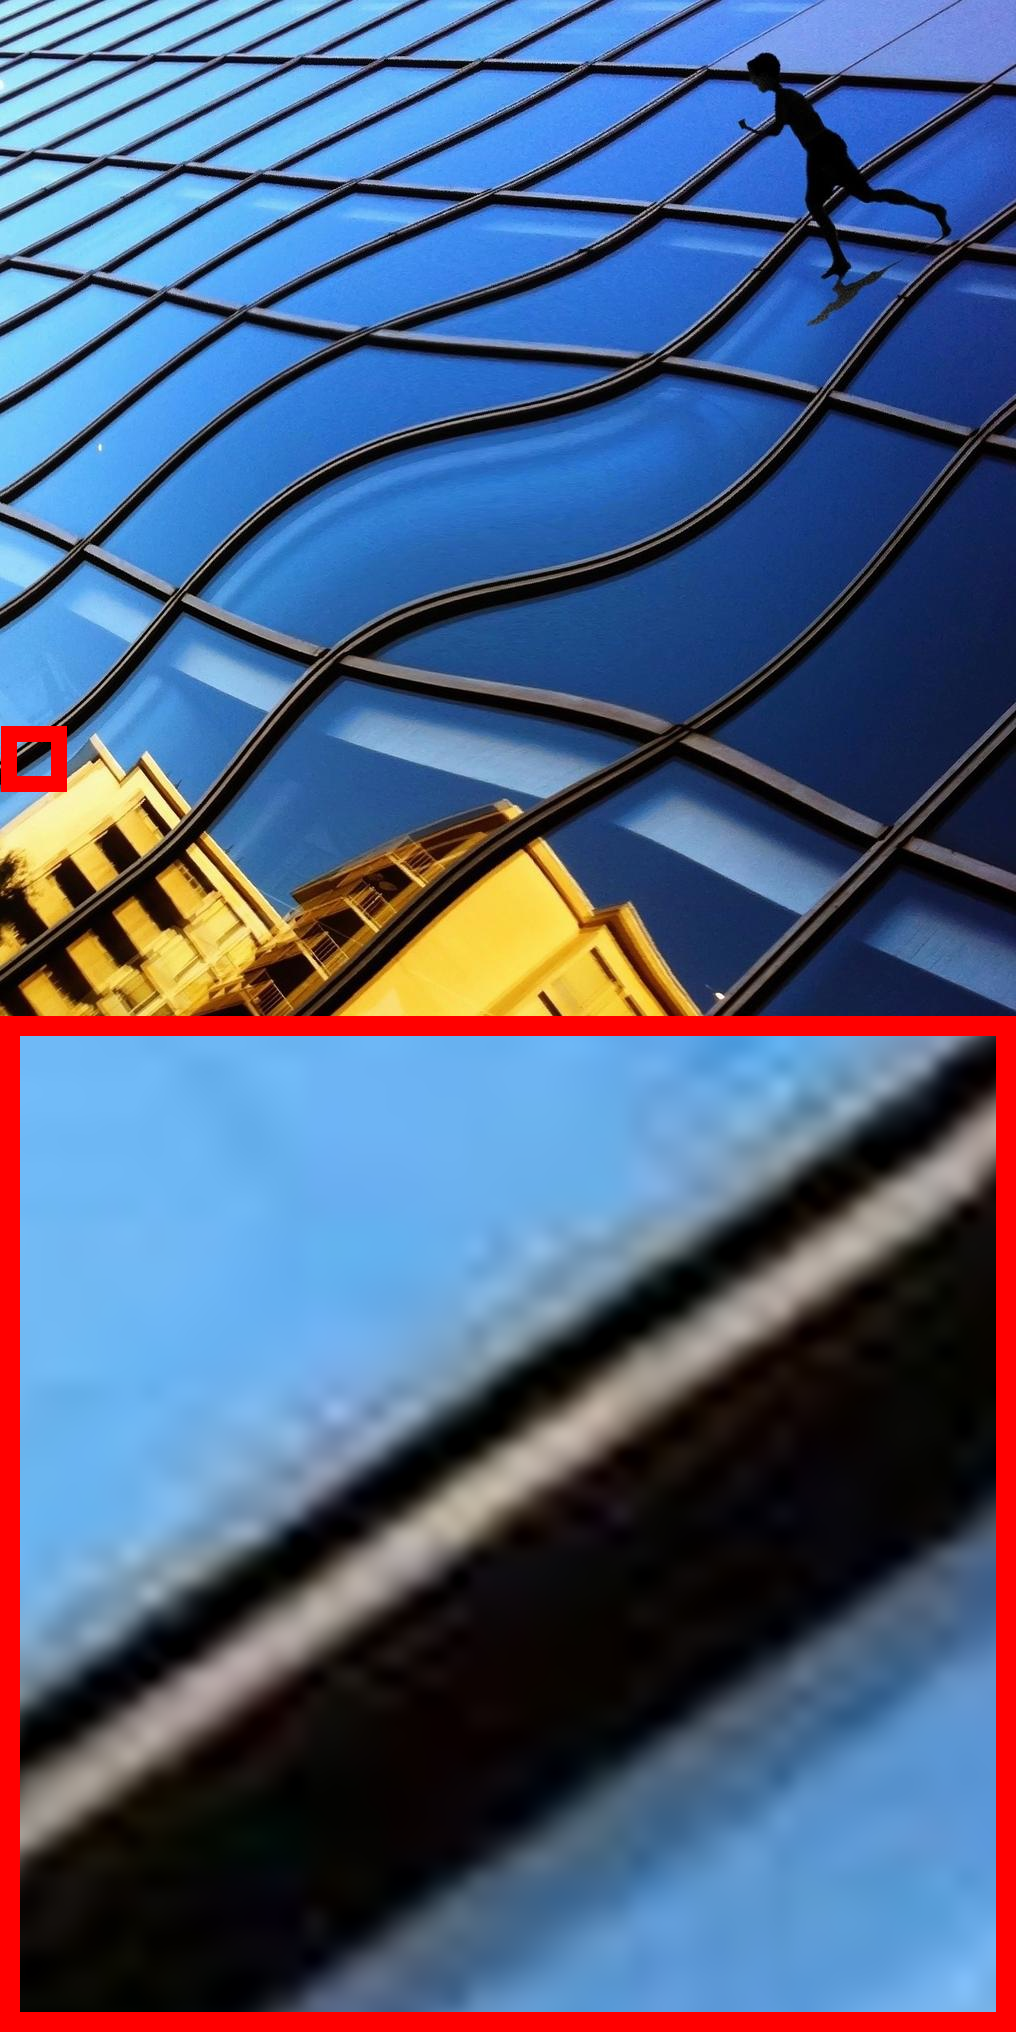
\includegraphics[width=0.18\textwidth]{img_082_1_w.png} &
%\graphicspath{{figs/}}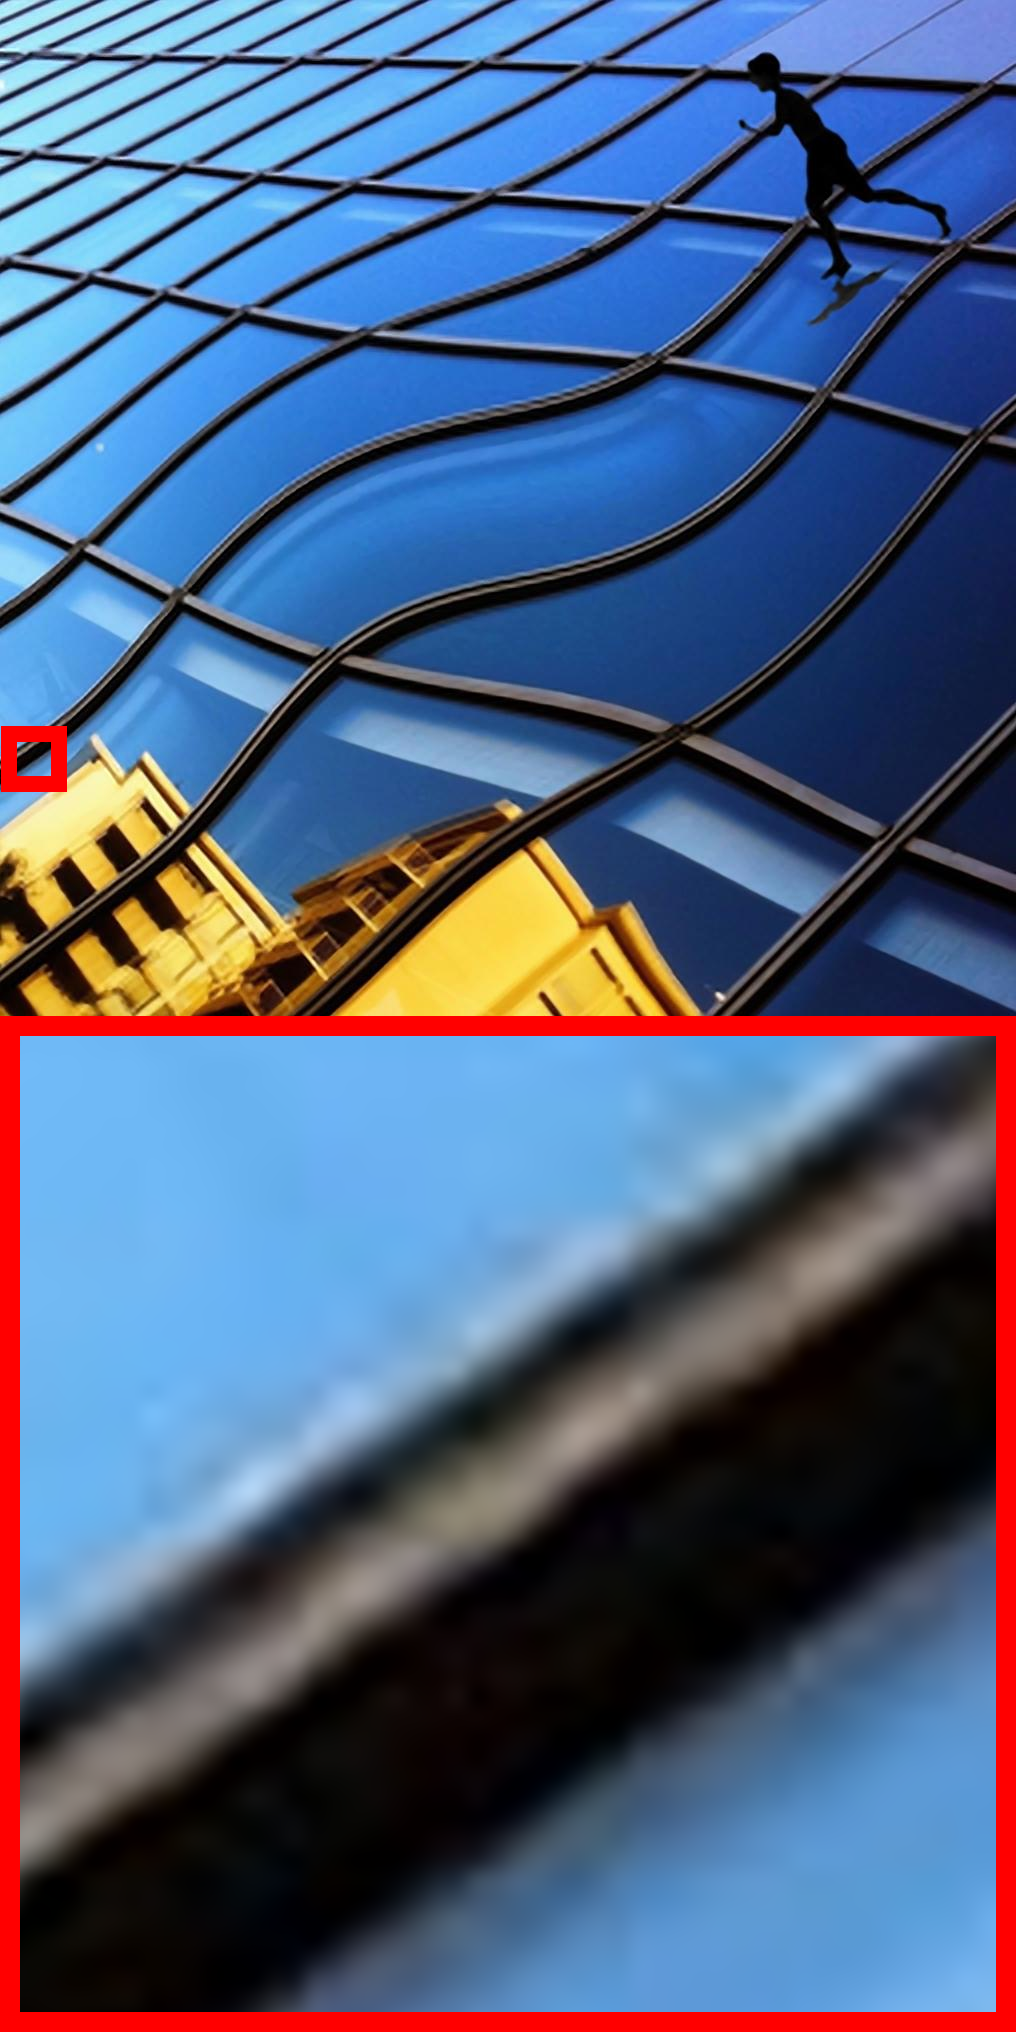
\includegraphics[width=0.18\textwidth]{img_082_6_w.png} &
%\graphicspath{{figs/}}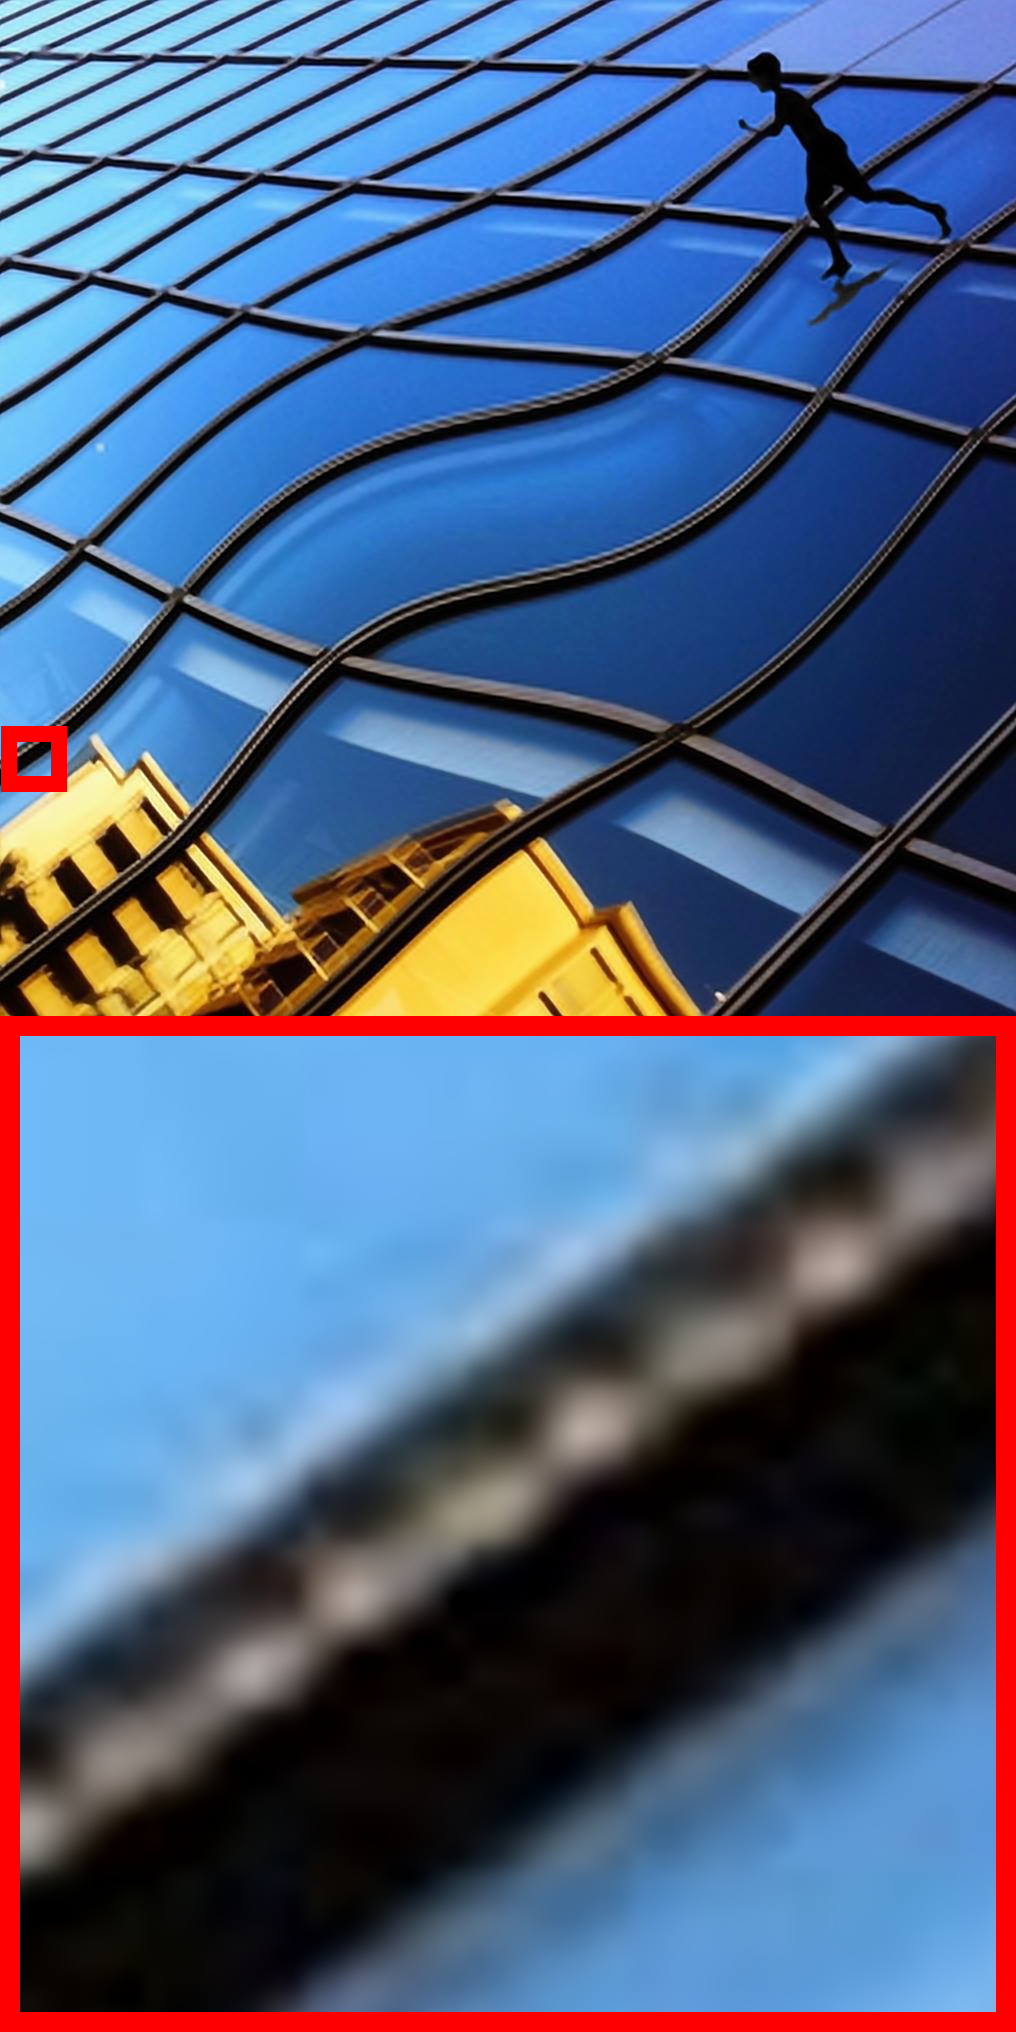
\includegraphics[width=0.18\textwidth]{img_082_7_w.png} &
%\graphicspath{{figs/}}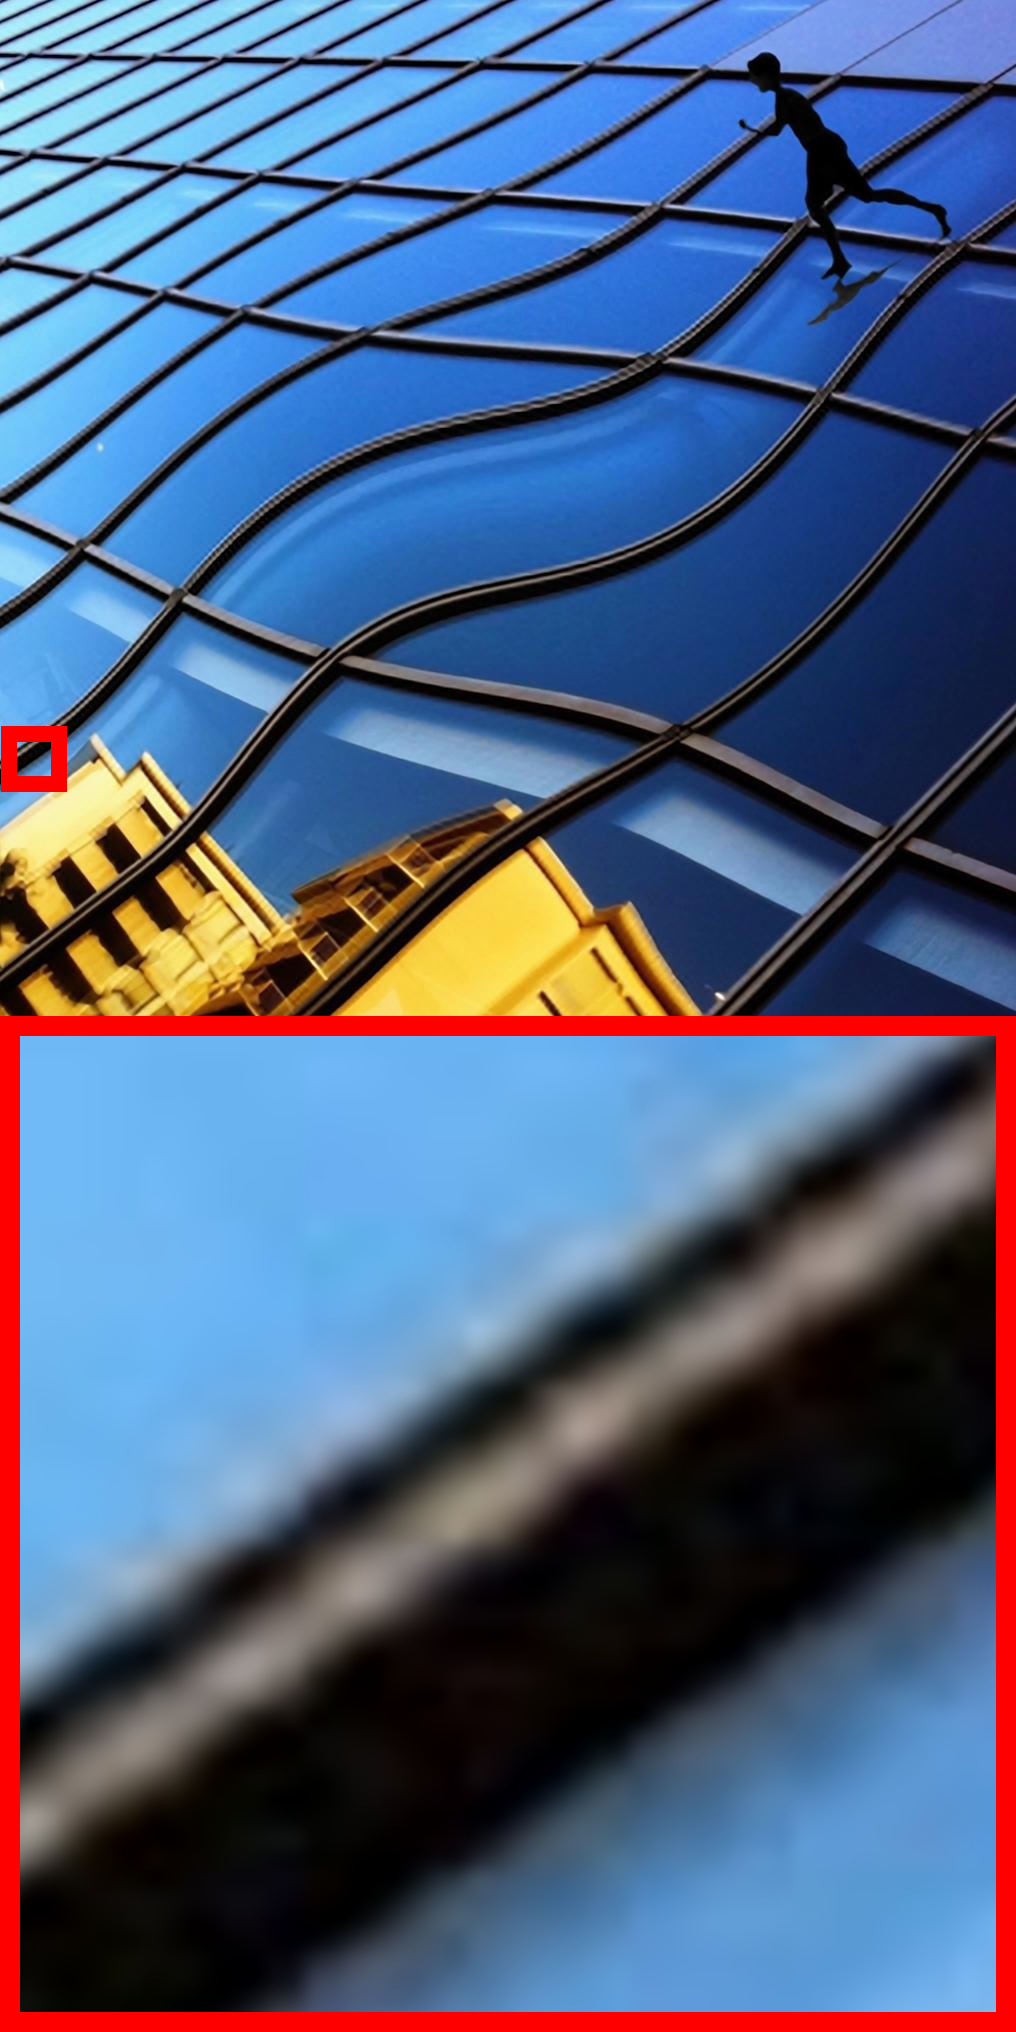
\includegraphics[width=0.18\textwidth]{img_082_10_w.png} &
%\graphicspath{{figs/}}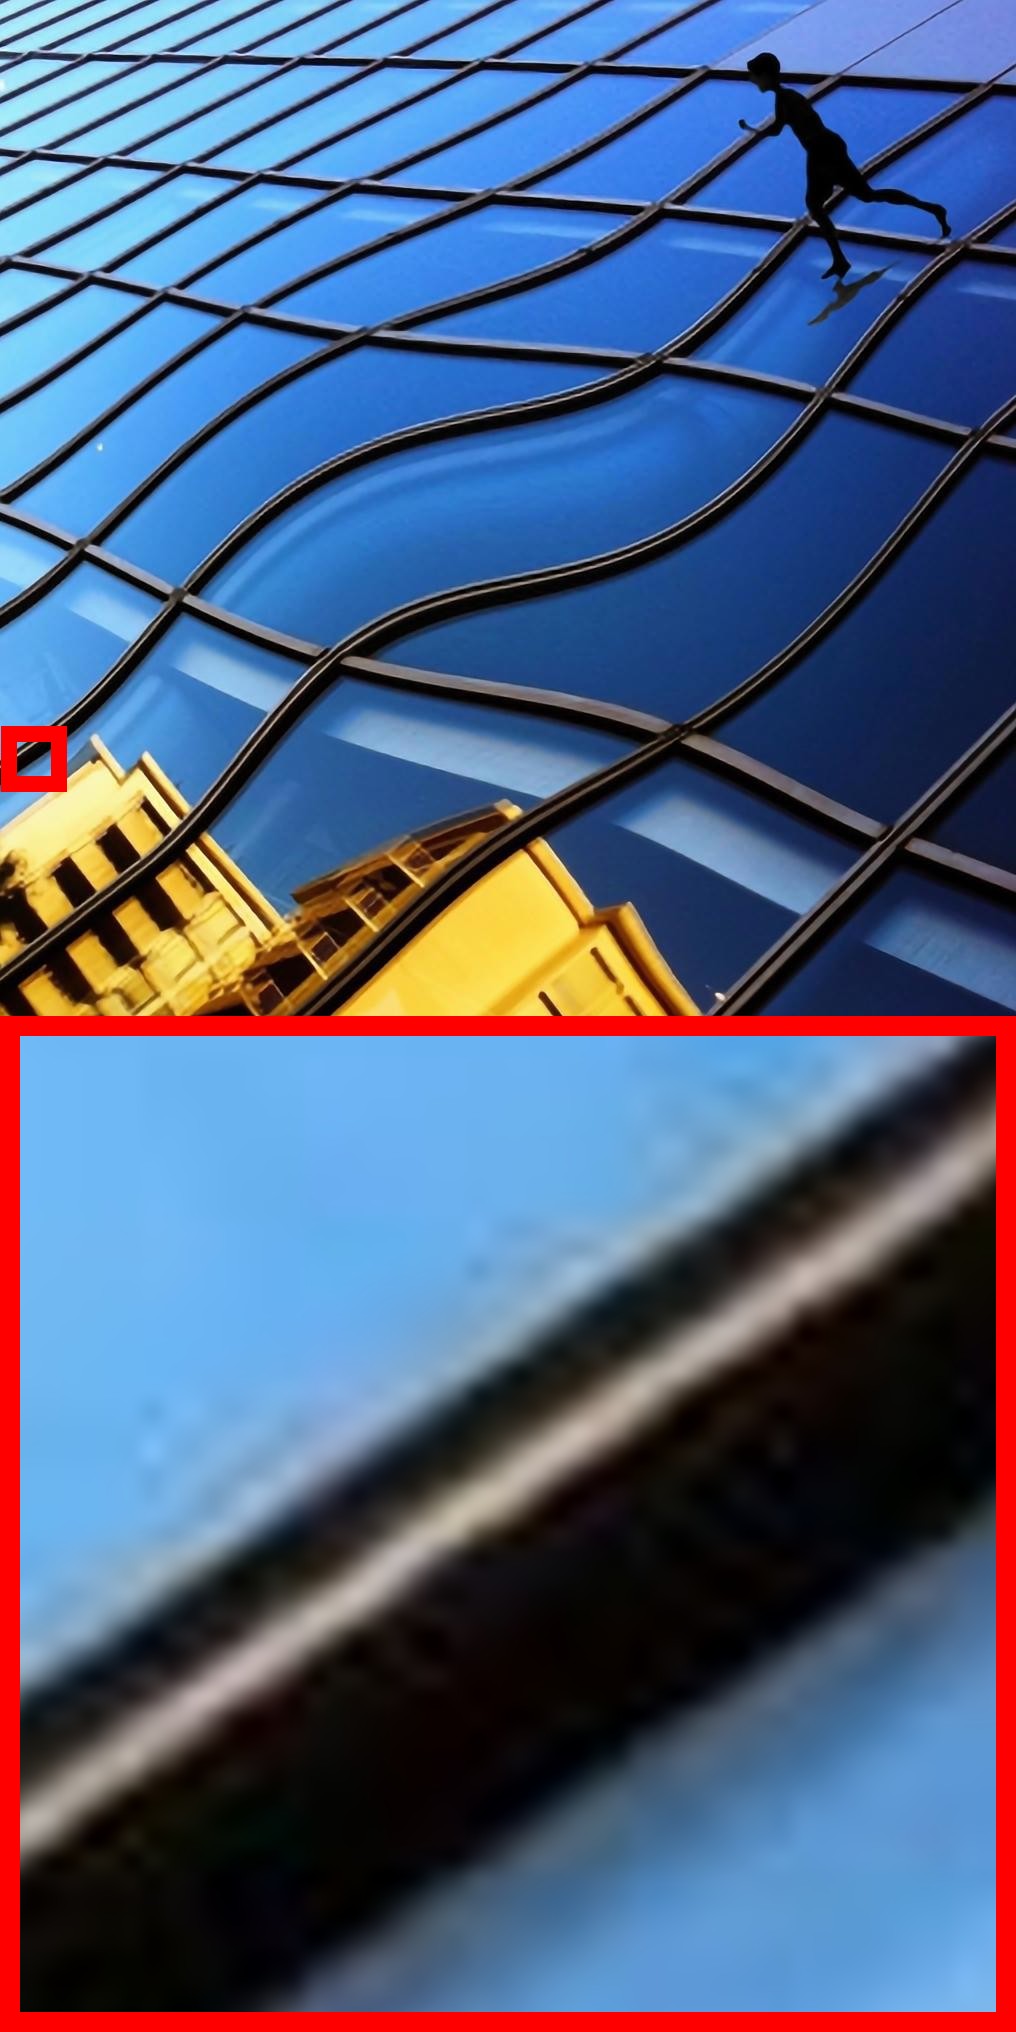
\includegraphics[width=0.18\textwidth]{img_082_9_w.png} 
%\\
%Original / PSNR (dB) &A+ / 29.84 &SRCNN / 29.20 &Huang et al. / 30.17 &RCN (Ours) / 30.86 \\
%\end{tabular}
%\end{center}
%\vspace{-.5cm}
%\caption{Super-resolution results (Urban100) with scale factor $\times$4 Our result is visually pleasing. }\label{fig:c1}
%\end{figure*}
%
%\begin{figure*}
%\begin{center}
%\begin{tabular}{cccc}
%\graphicspath{{figs/}}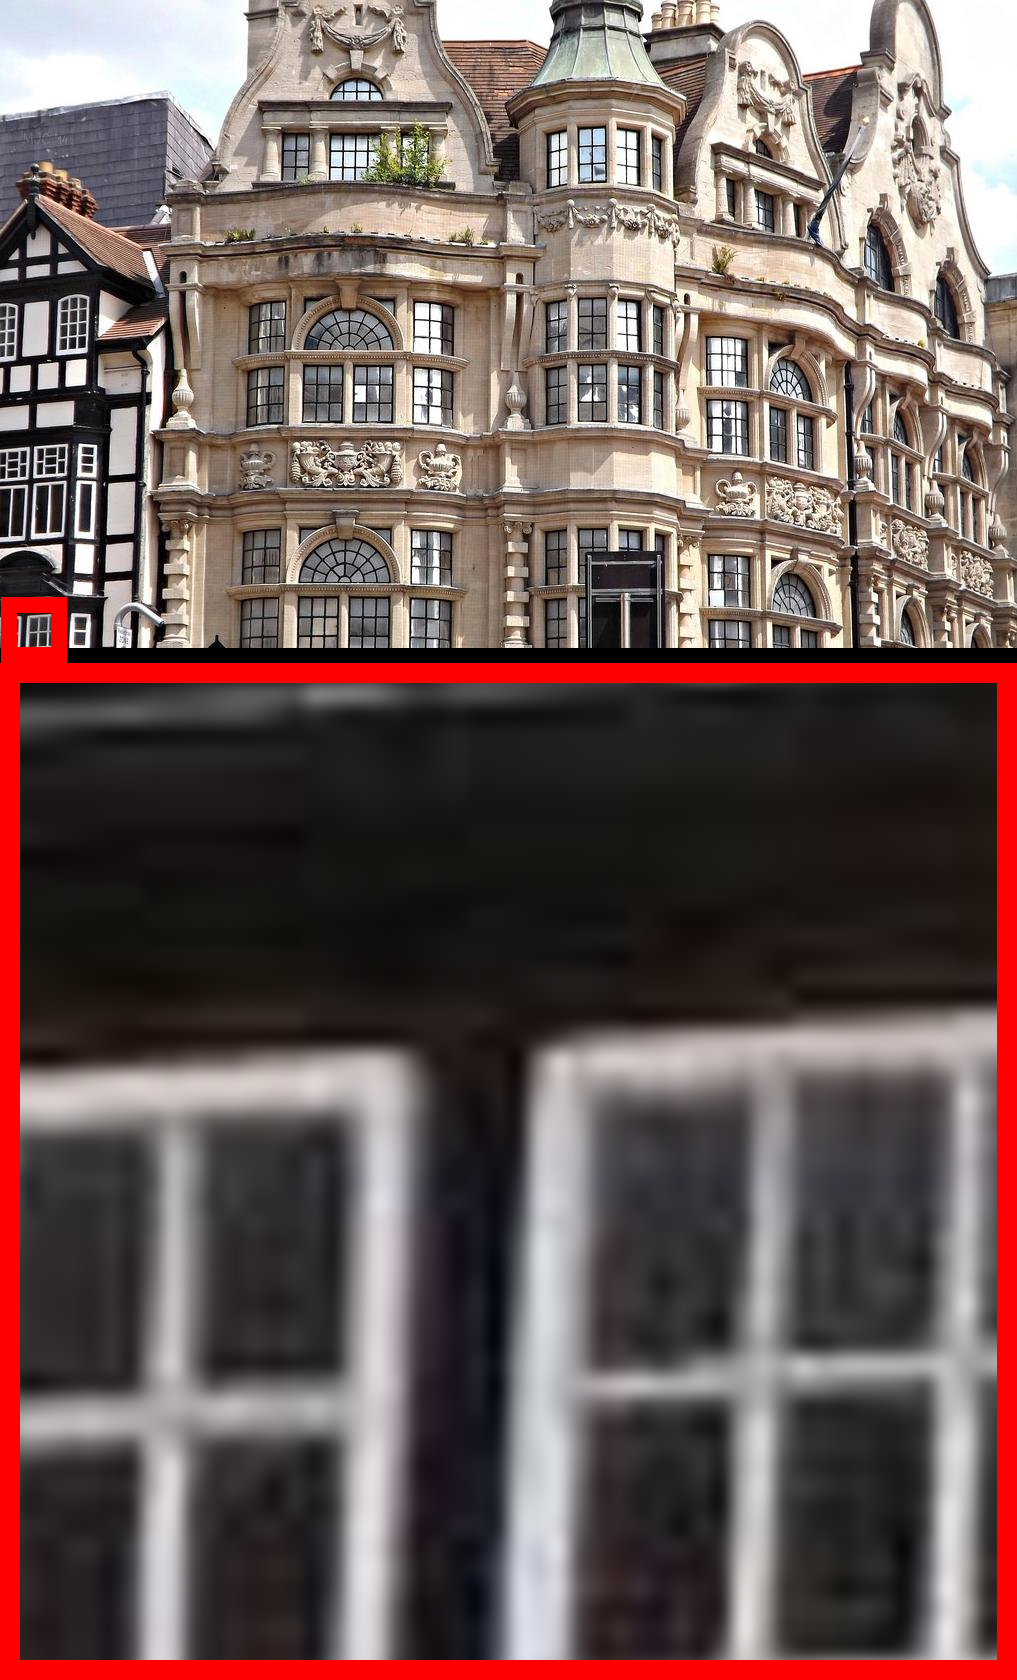
\includegraphics[width=0.23\textwidth]{img_053_1_w.png} &
%\graphicspath{{figs/}}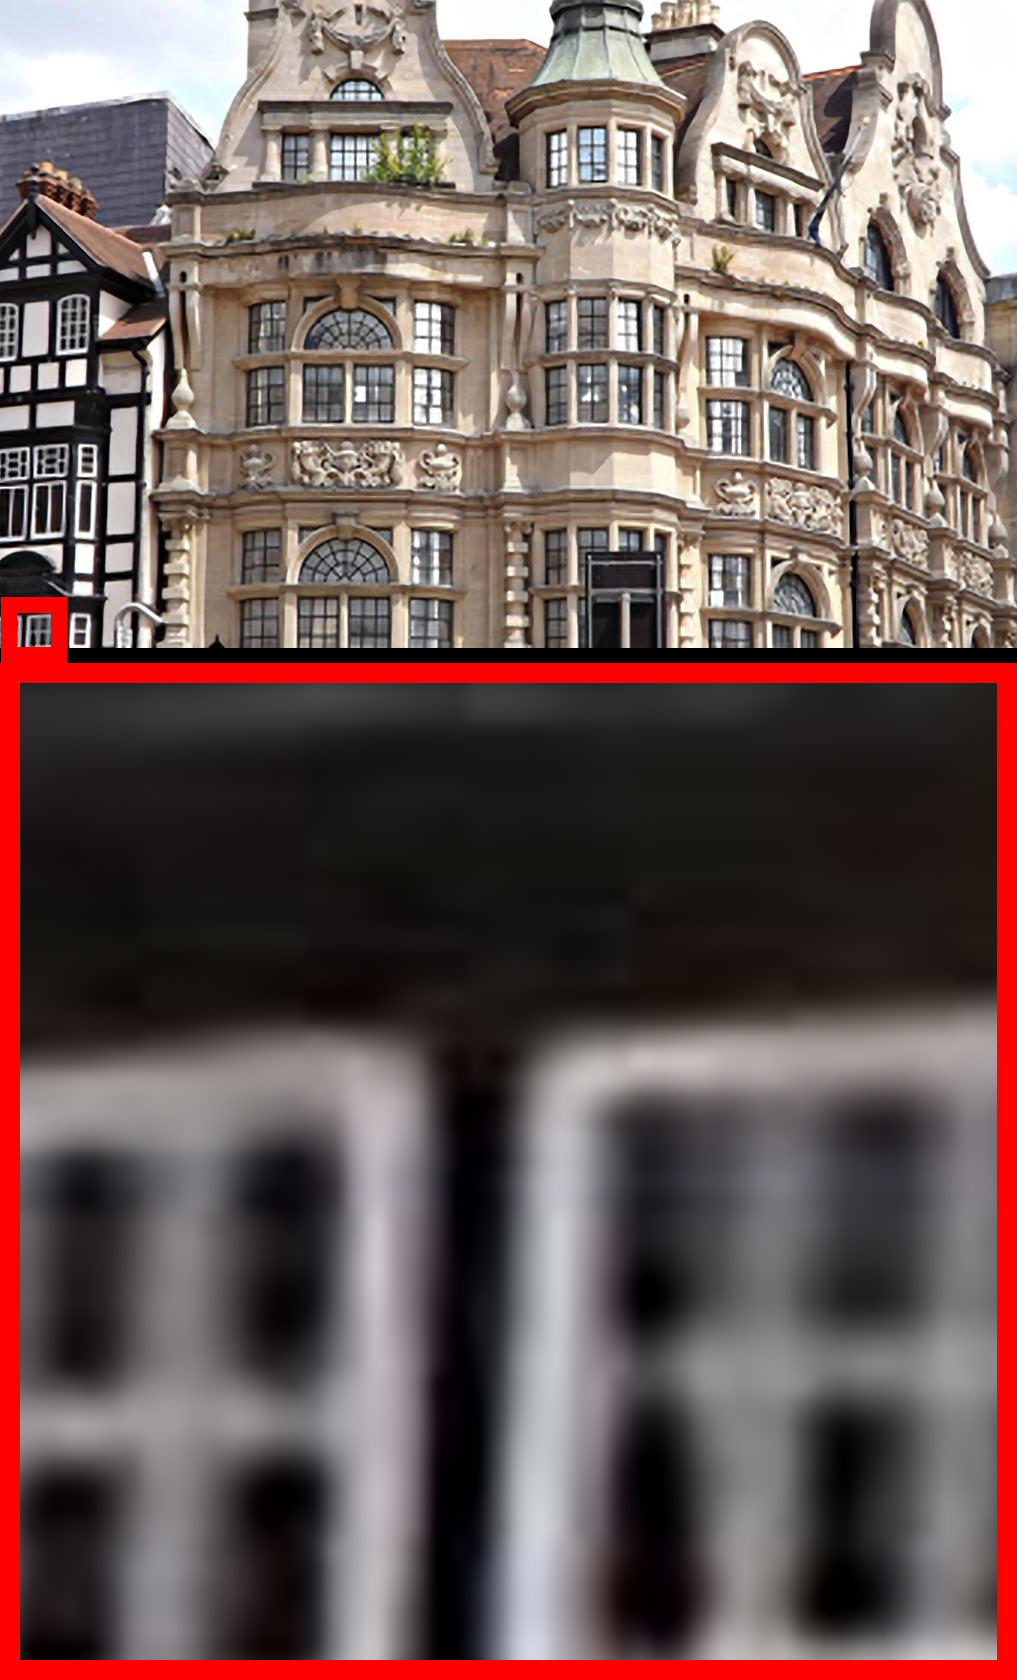
\includegraphics[width=0.23\textwidth]{img_053_6_w.png} &
%\graphicspath{{figs/}}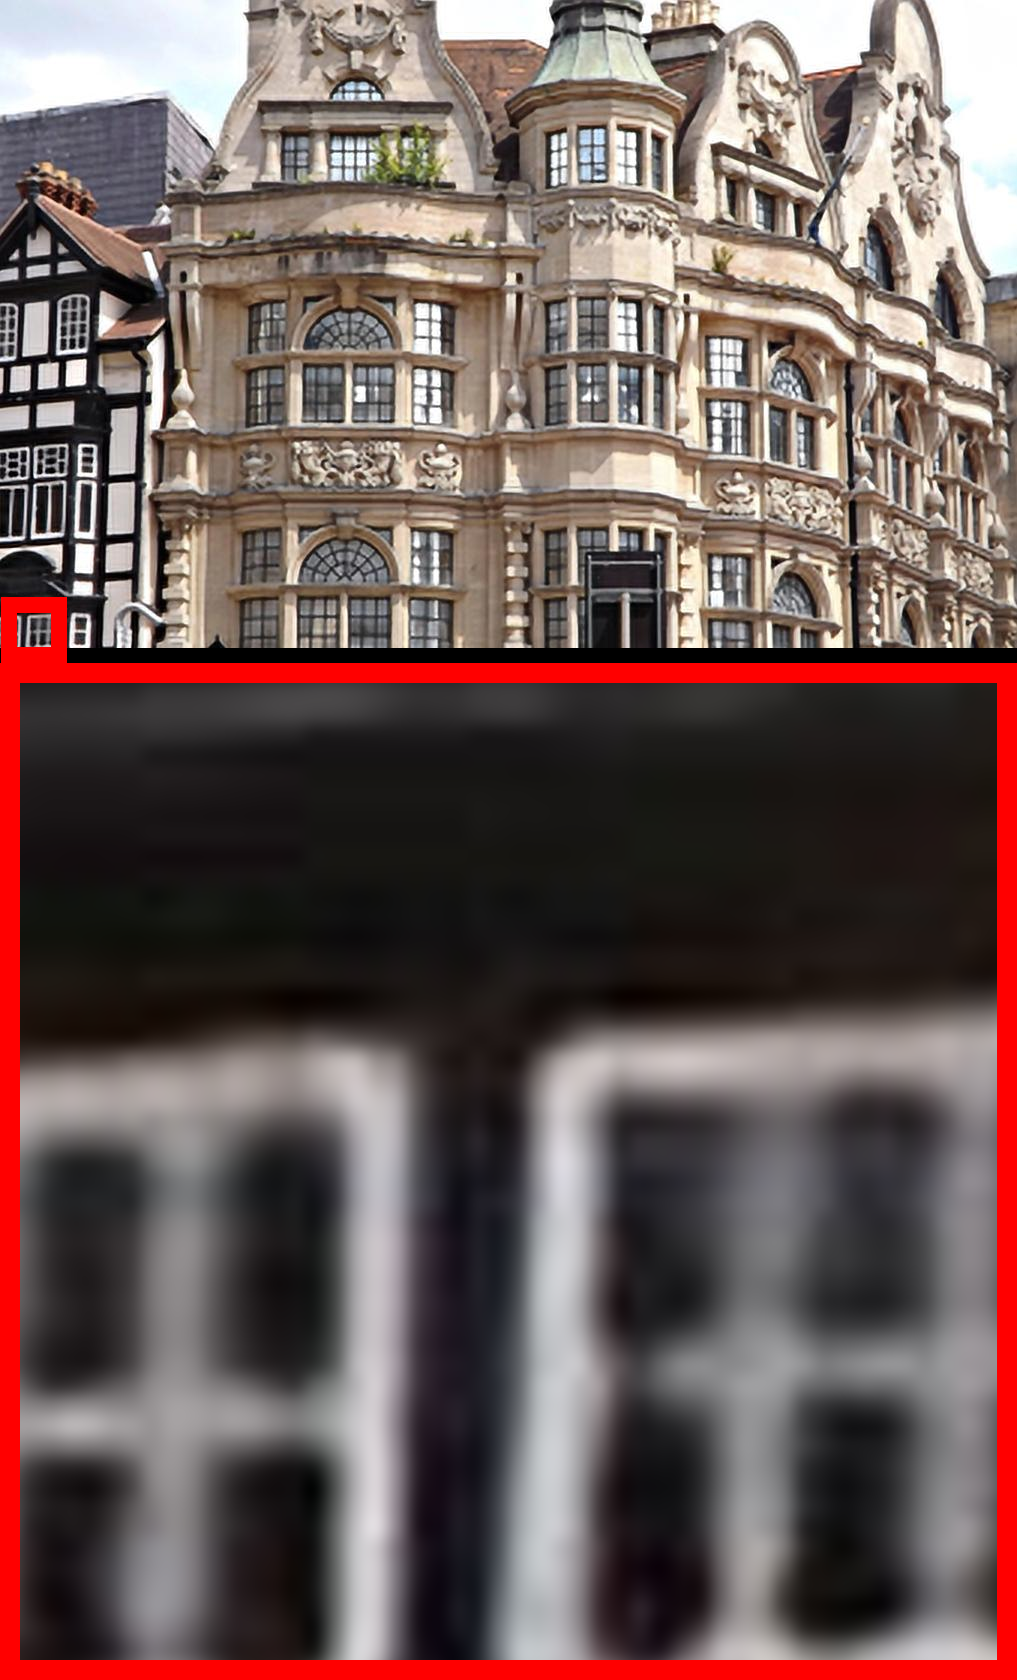
\includegraphics[width=0.23\textwidth]{img_053_7_w.png} &
%\graphicspath{{figs/}}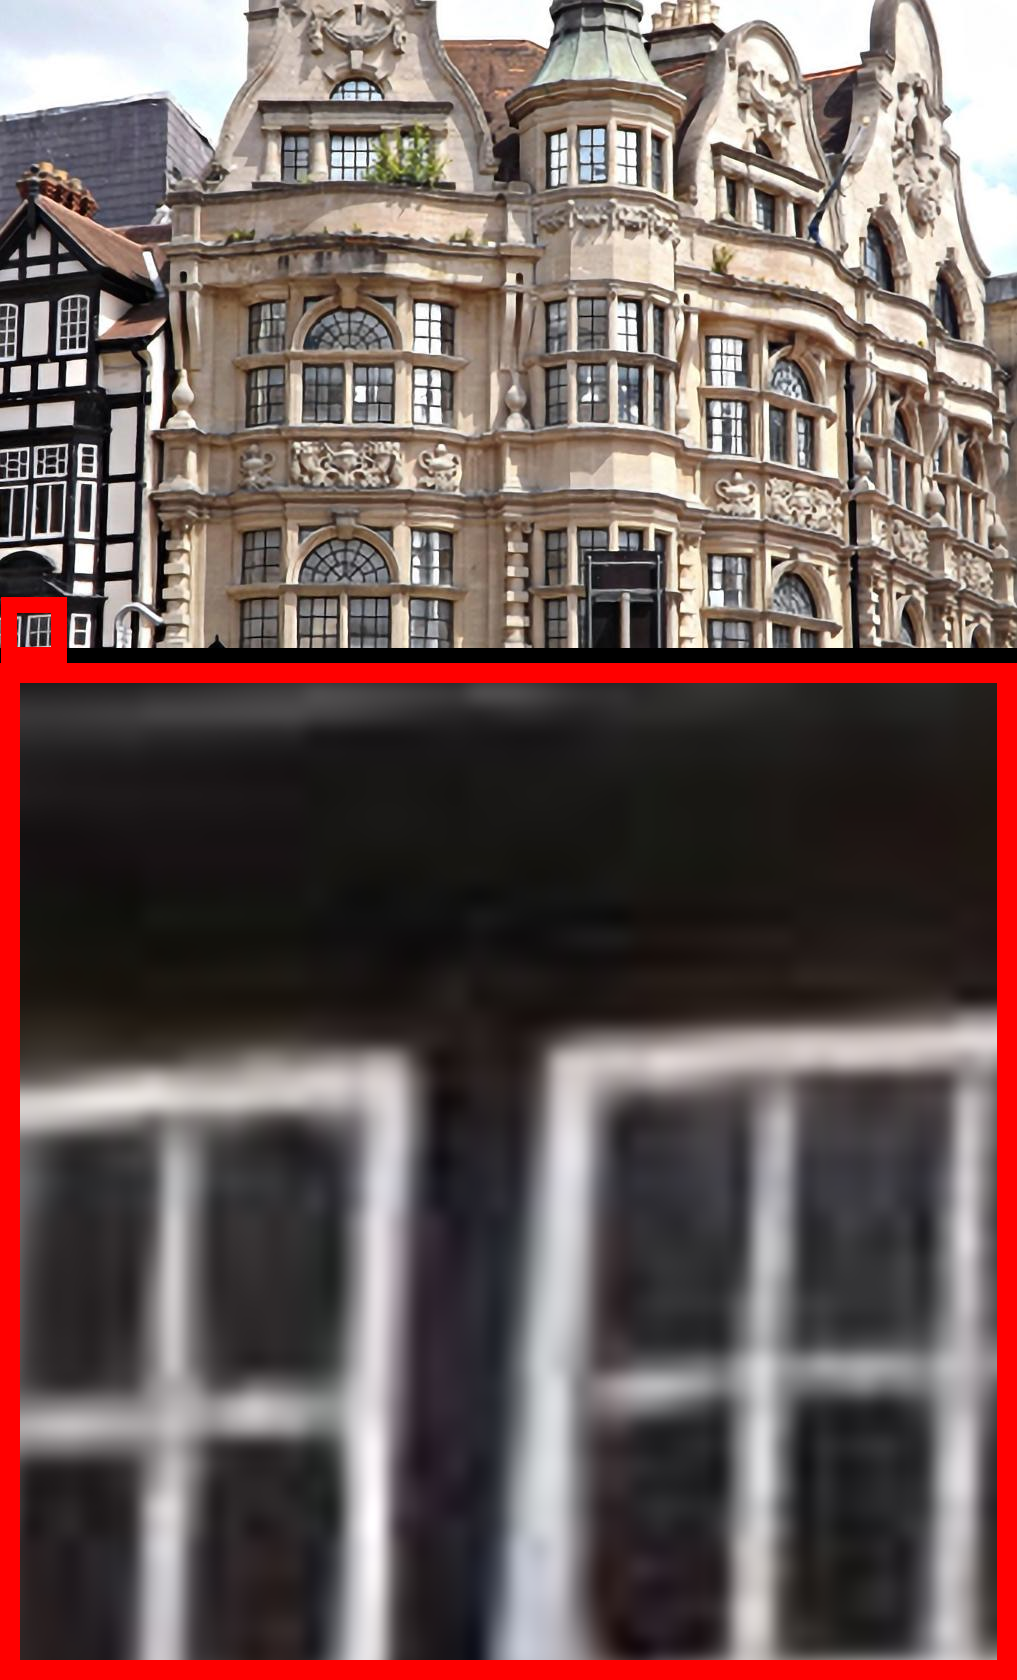
\includegraphics[width=0.23\textwidth]{img_053_9_w.png} 
%\\
%Original / PSNR (dB) &A+ / 22.31 &SRCNN / 22.34 &RCN (Ours) / 23.13 \\
%\end{tabular}
%\end{center}
%\vspace{-.5cm}
%\caption{Super-resolution results (Urban100) with scale factor $\times$3. Our result is visually pleasing.}\label{fig:c2}
%\end{figure*}
%
%
%\begin{figure*}
%\begin{center}
%\begin{tabular}{cccc}
%\graphicspath{{figs/}}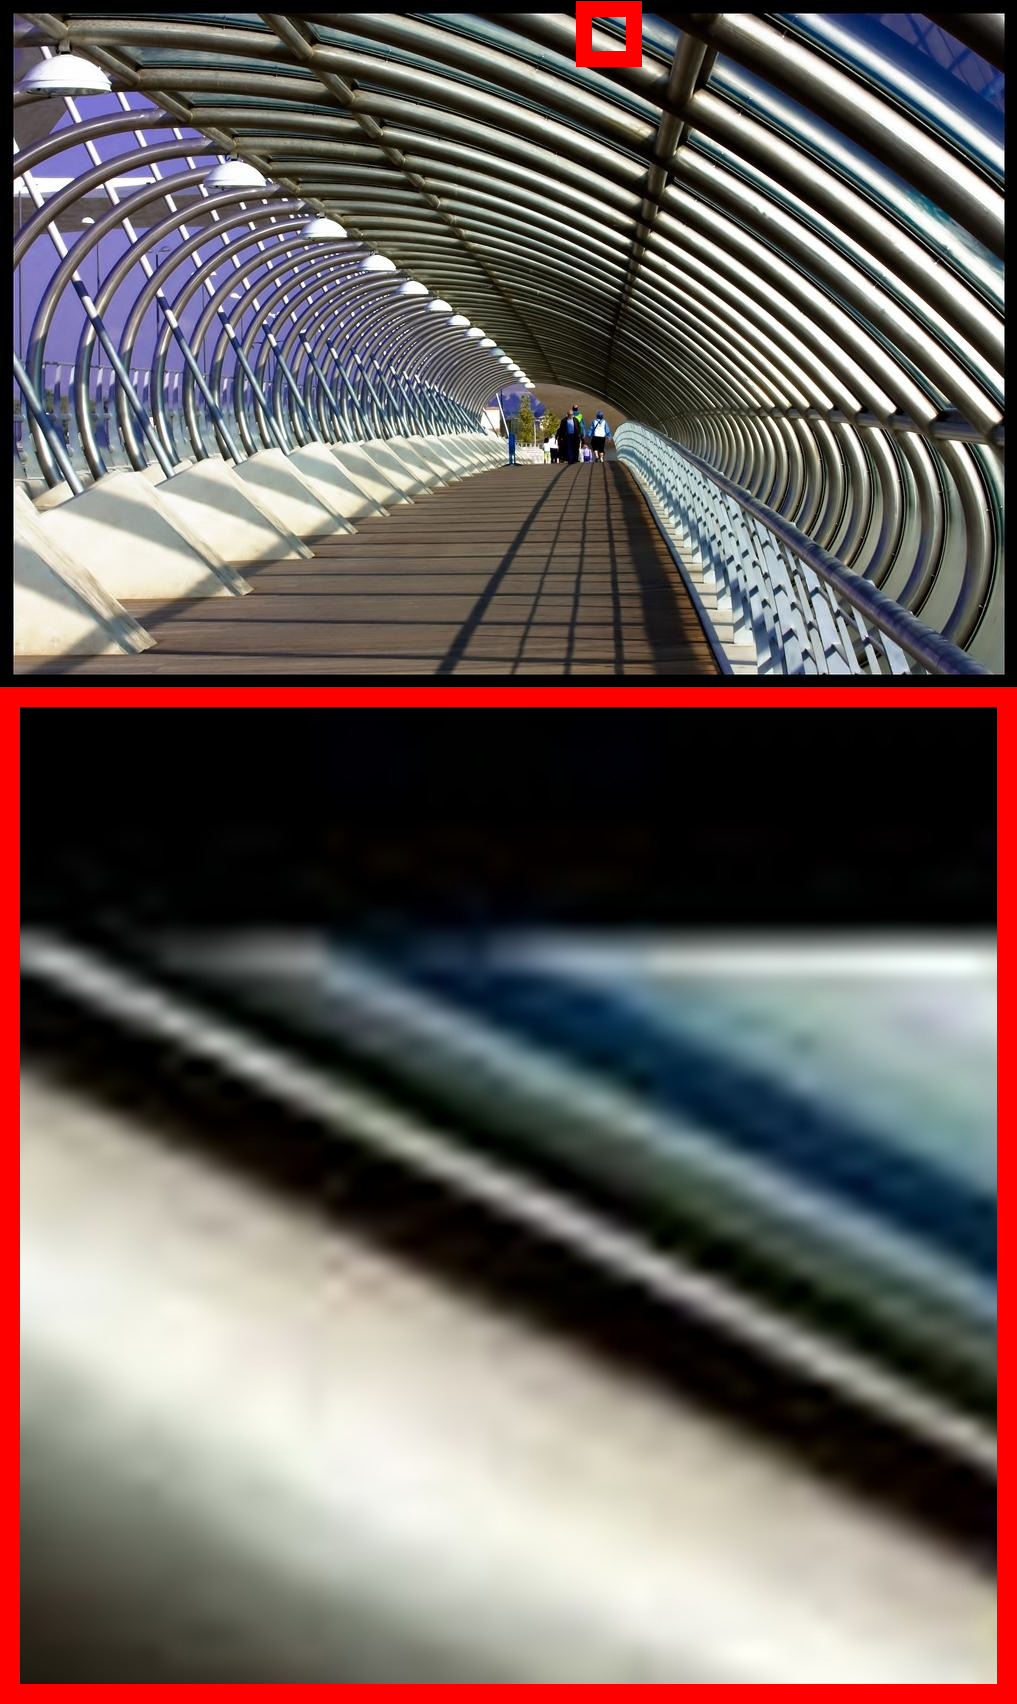
\includegraphics[width=0.23\textwidth]{img_058_1_w.png} &
%\graphicspath{{figs/}}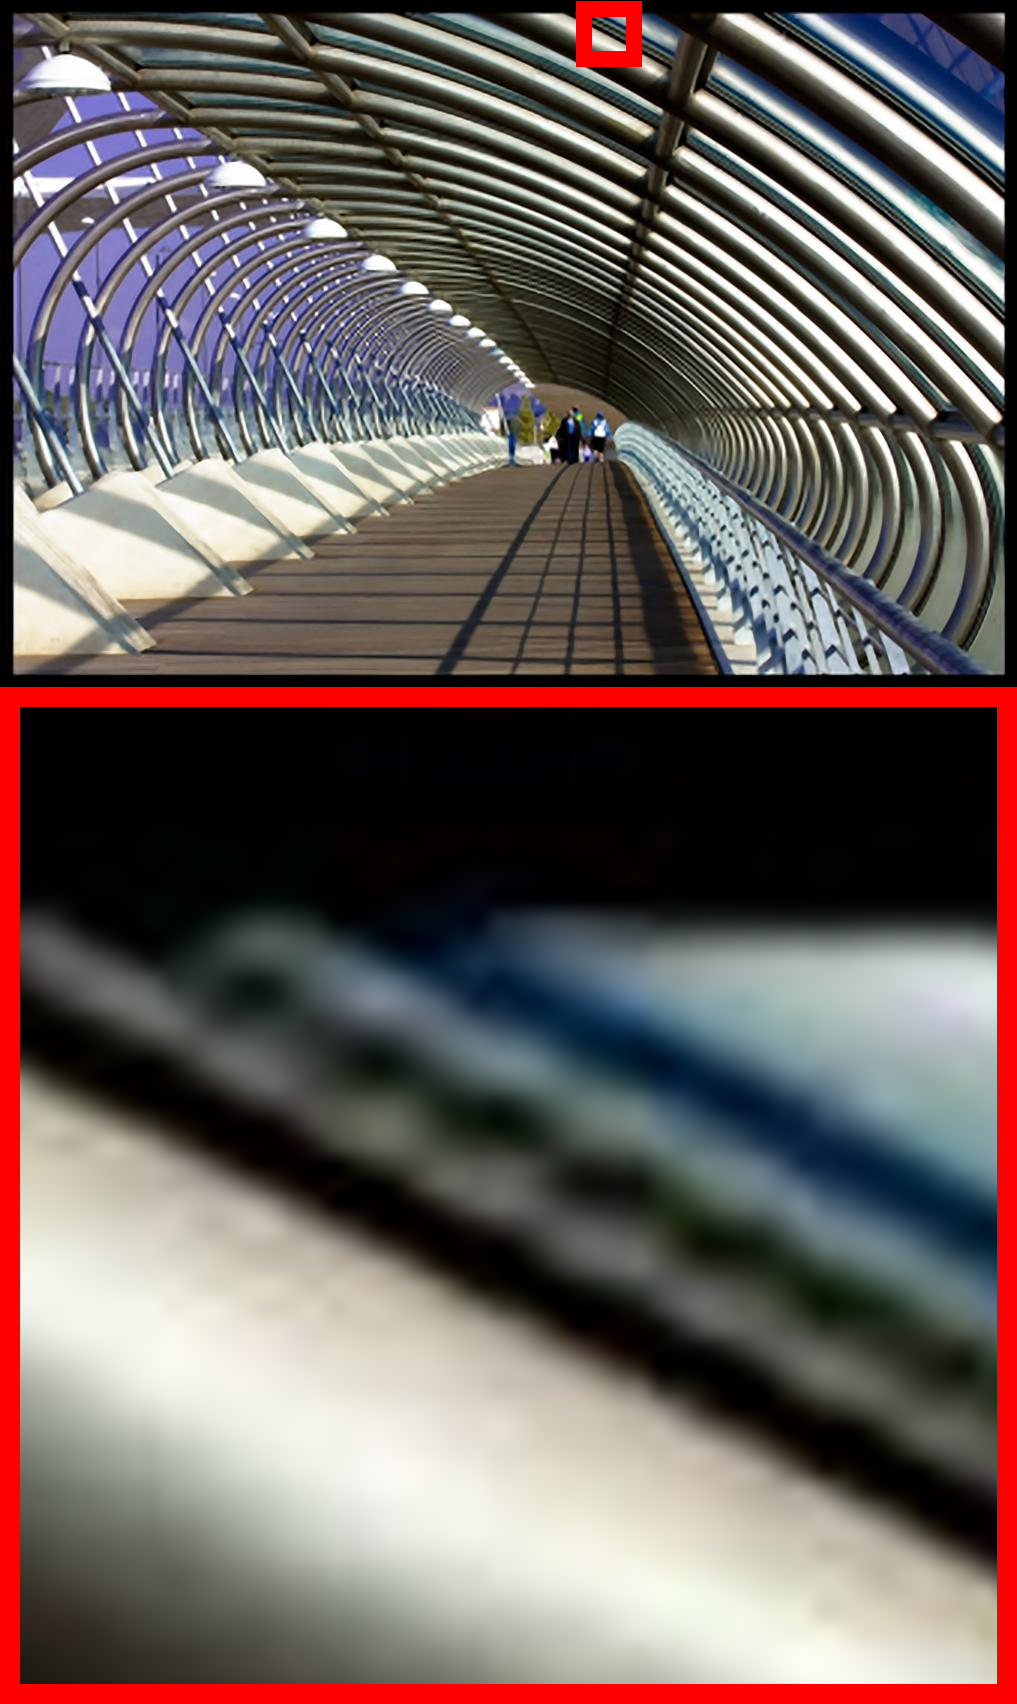
\includegraphics[width=0.23\textwidth]{img_058_6_w.png} &
%\graphicspath{{figs/}}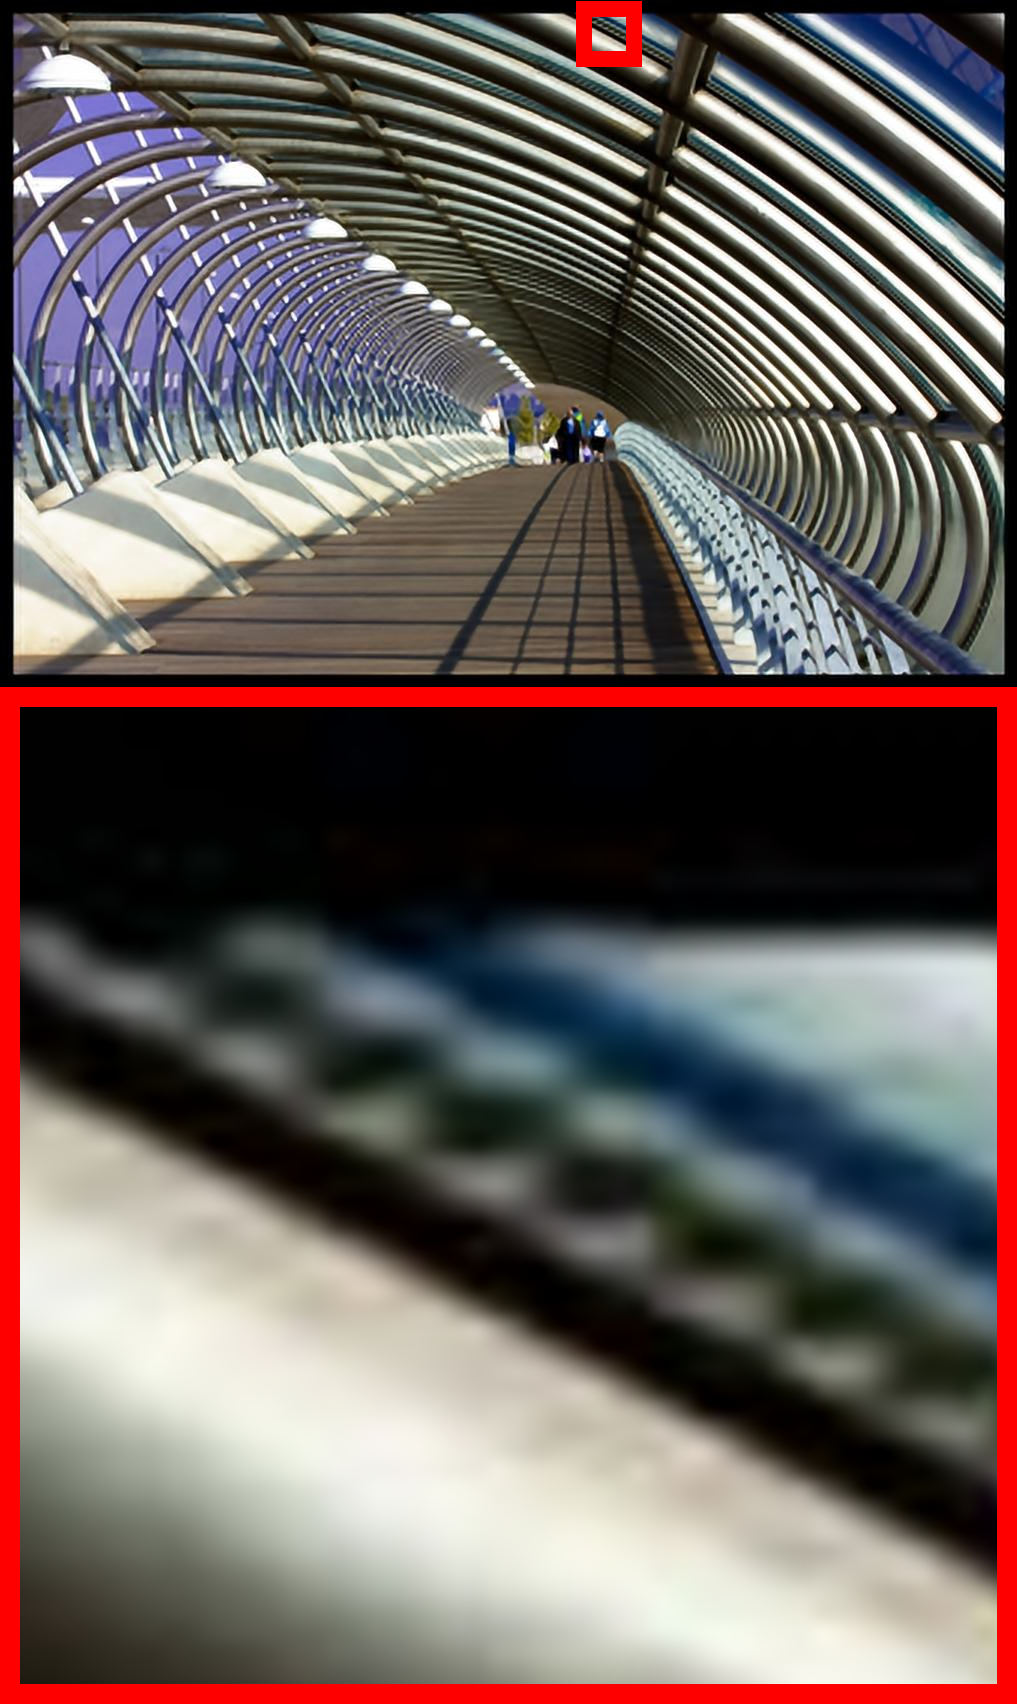
\includegraphics[width=0.23\textwidth]{img_058_7_w.png} &
%\graphicspath{{figs/}}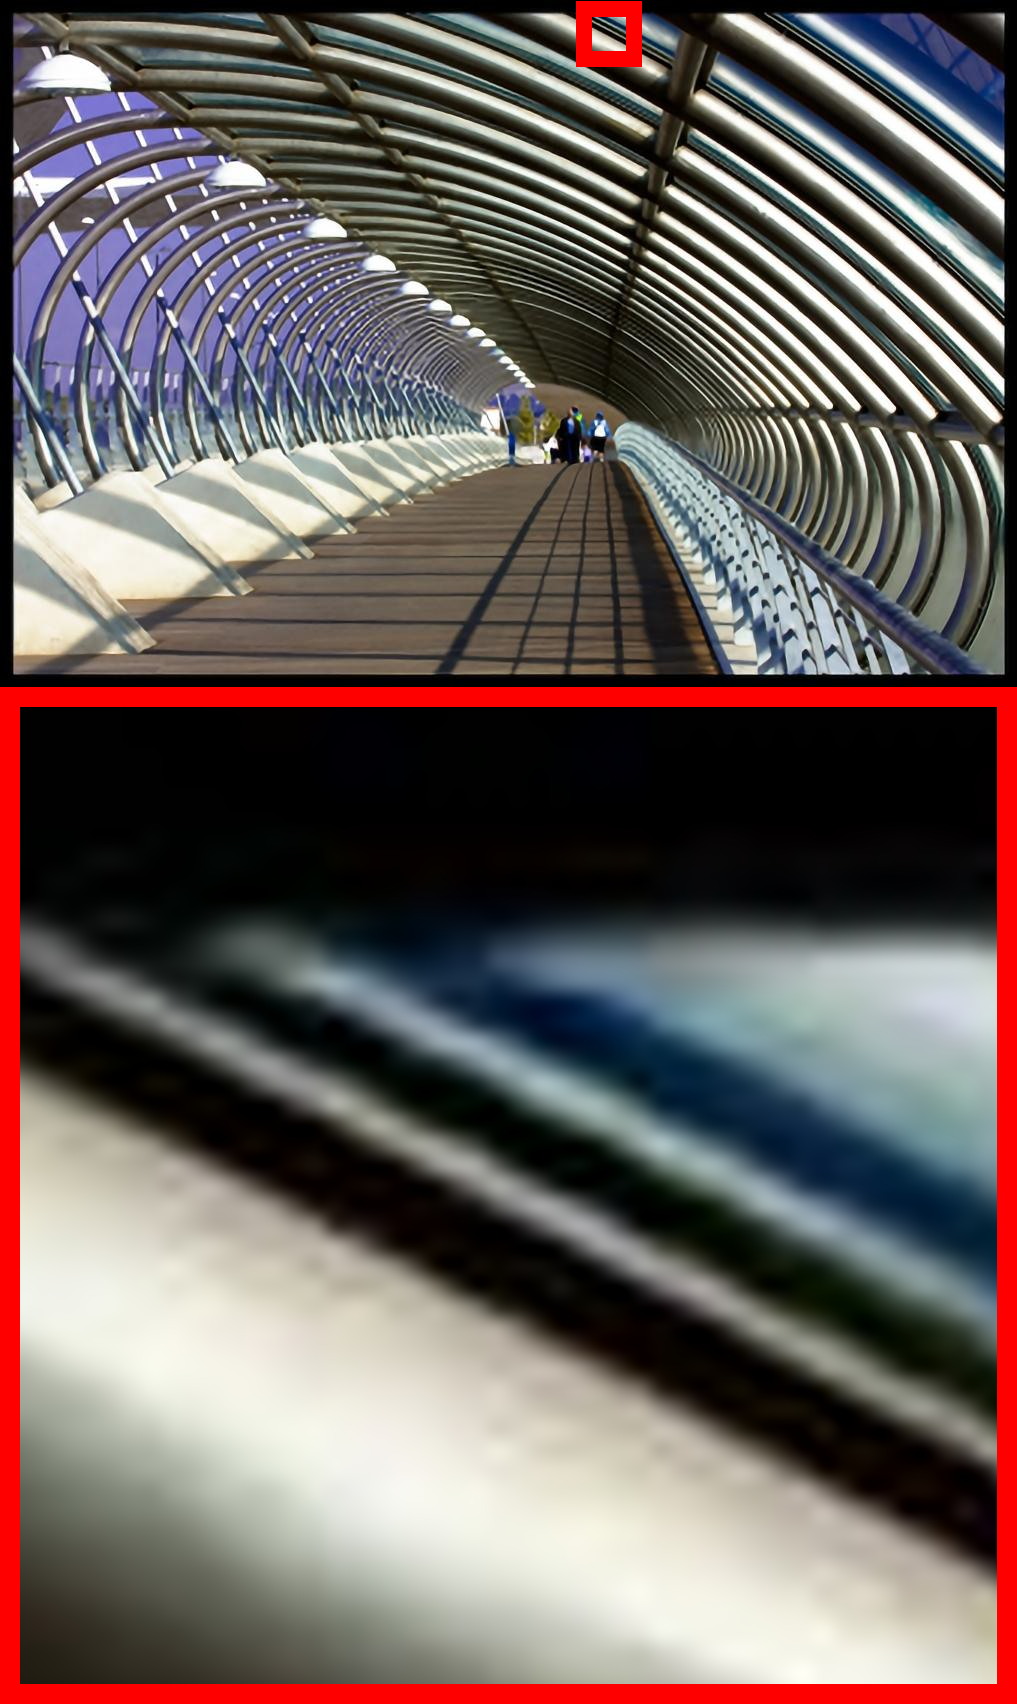
\includegraphics[width=0.23\textwidth]{img_058_9_w.png} 
%\\
%Original / PSNR (dB) &A+ / 25.87 &SRCNN / 25.76 &RCN (Ours) / 26.57 \\
%\end{tabular}
%\end{center}
%\vspace{-.5cm}
%\caption{Super-resolution results (Urban100) with scale factor $\times$3. Our result is visually pleasing.}\label{fig:c3}
%\end{figure*}
%
%\subsection{High Depths for Large Contexts}
%In this section, we study the depth of a convolutional neural network (CNN) in the context of super-resolution. We first start with the definition of receptive field in a CNN. 
%
%CNNs exploit spatially-local correlation by enforcing a local connectivity pattern between neurons of adjacent layers \cite{Bengio-et-al-2015-Book}. In other words, hidden units in layer $m$ take as input a subset of units in layer $m-1$. They form spatially contiguous receptive fields (Figure \ref{fig:receptive_field}).
%
%Imagine that layer $m-1$ is the input image. In the figure, units in layer $m$ have receptive fields of 3$\times$3 in the input and are thus only connected to 9 adjacent neurons in the input layer. Units in layer $m+1$ have a similar connectivity with the layer below. We say that their receptive field with respect to the layer below is 3$\times$3, but their receptive field with respect to the input is larger (5$\times$5). Each unit is unresponsive to variations outside of its receptive field with respect to the input. The architecture thus ensures that the learned filters produce the strongest response to a spatially local input pattern.
%
%However, as shown above, stacking many such layers leads to filters that become increasingly “global” (i.e. responsive to a larger region of pixel space). For example, the unit in hidden layer $m+1$ can encode a non-linear feature of 5$\times$5 (in terms of image pixel space).
%
%In this work, we use small filters of the same size 3$\times$3 for all layers. For the first layer, its receptive field is of size 3$\times$3. For the next layers, the size of its receptive field increases by 2 in both height and width. For depth $M$ network, its receptive field has size $(2M+1)\times(2M+1)$. Its size is proportional to the depth.
%
%In the task of SR, this corresponds to the amount of contextual information that can be exploited to infer high-frequency components. Large receptive field means the network can use more context from large image region to predict details of an image. As SR is an ill-posed inverse problem, collecting and analyzing more neighbor pixels give more clues. For example, if there are some image patterns entirely contained in a receptive field, it is plausible that this pattern is recognized and used to super-resolve the image. 
%
%We now experimentally show that very deep networks significantly improve performance.  Since our layers are of the same type, we train and test networks of depth ranging from 5 to 20 (only counting weight layers excluding nonlinearity layers). 
%
%In Figure \ref{fig:depth}, we show the results. In most cases, performance increases as depth increases. The exception is scale factor 2. As depth increases, performance on scale factors 3 and 4 improve rapidly. Since we use Euclidean loss, it tends to correct severe errors first, which are more prevalent in high scale factors. Different loss functions can be explored to balance the importance between scales and these are left as a future work. 
%
%\begin{table*}
%\footnotesize
%\begin{center}
%\begin{tabular}{ |c|c|c|c|c|c|c|c|c|c| }
%\hline
%\multirow{2}{*}{Dataset} & \multirow{2}{*}{Scale} & {Bicubic} & {A+} & {SRCNN} & {Huang et al.} & {RCN} & {RCN-291} & {RCN+} & {RCN-291+ (Ours)}\\ 
%
% &  & PSNR/Time & PSNR/Time & PSNR/Time & PSNR/Time & PSNR/Time & PSNR/Time & PSNR/Time & PSNR/Time\\ 
%\hline
%\hline
%\multirow{3}{*}{Set5}
%& $\times$2& 33.66 / - & 36.55 / 0.44& 36.66 / 2.12& -& 37.06 / 0.31& \color{blue} 37.38 / 0.15& 37.24 / 0.18& \color{red} 37.53 / 0.19\\
%& $\times$3& 30.39 / - & 32.59 / 0.23& 32.75 / 2.13& -& 33.27 / 0.22& 33.42 / 0.15& \color{blue} 33.50 / 0.18& \color{red} 33.67 / 0.19\\
%& $\times$4& 28.42 / - & 30.28 / 0.16& 30.49 / 2.21& -& 30.95 / 0.22& 31.09 / 0.15& \color{blue} 31.22 / 0.18& \color{red} 31.35 / 0.19\\
%\hline
%\hline
%\multirow{3}{*}{Set14}
%& $\times$2& 30.23 / - & 32.28 / 0.92& 32.45 / 3.79& -& 32.61 / 0.32& \color{blue} 32.84 / 0.21& 32.77 / 0.26& \color{red} 33.04 / 0.27\\
%& $\times$3& 27.54 / - & 29.13 / 0.48& 29.30 / 3.78& -& 29.48 / 0.32& 29.63 / 0.21& \color{blue} 29.64 / 0.26& \color{red} 29.77 / 0.27\\
%& $\times$4& 26.00 / - & 27.32 / 0.34& 27.50 / 3.80& -& 27.71 / 0.32& 27.85 / 0.21& \color{blue} 27.91 / 0.26& \color{red} 28.01 / 0.27\\
%\hline
%\hline
%\multirow{3}{*}{Urban100}
%& $\times$2& 26.61 / - & 28.57 / 3.15& 28.82 / 12.78& -& 29.22 / 0.76& \color{blue} 29.52 / 0.51& 29.41 / 0.67& \color{red} 29.76 / 0.68\\
%& $\times$3& 24.36 / - & 25.82 / 1.68& 25.99 / 12.85& -& 26.35 / 0.76& 26.52 / 0.51& \color{blue} 26.53 / 0.67& \color{red} 26.76 / 0.68\\
%& $\times$4& 23.07 / - & 24.22 / 1.17& 24.40 / 12.60& 24.55 / -& 24.62 / 0.77& 24.78 / 0.51& \color{blue} 24.82 / 0.67& \color{red} 24.99 / 0.68\\
%\hline
%\hline
%\multirow{3}{*}{B100}
%& $\times$2& 29.32 / - & 30.77 / 0.58& 30.89 / 2.43& 30.70 / -& 31.02 / 0.25& \color{blue} 31.21 / 0.17& 31.13 / 0.21& \color{red} 31.30 / 0.22\\
%& $\times$3& 27.15 / - & 28.18 / 0.31& 28.28 / 2.48& 28.10 / -& 28.42 / 0.25& \color{blue} 28.55 / 0.17& 28.52 / 0.21& \color{red} 28.64 / 0.22\\
%& $\times$4& 25.92 / - & 26.77 / 0.22& 26.84 / 2.39& 26.74 / -& 26.98 / 0.25& \color{blue} 27.10 / 0.17& 27.08 / 0.20& \color{red} 27.20 / 0.21\\
%\hline
%\end{tabular}
%\end{center}
%\caption{\textcolor{red}{PSNR for scale factor $\times$2, $\times$3 and $\times$4 on datasets `Set5', `Set14', `Urban100', and `B100'.} {\color{red} Red color} indicates the best performance and {\color{blue}blue color} indicates the second best one.} \label{table_all}
%\end{table*}
%
%%\begin{table*}
%%\small	
%%	\centering
%%	\caption{PSNR for scale factor $\times$3 for Set14. {\color{red}Red color} indicates the best performance and {\color{blue}{blue color}} indicates the second best one.}
%%	\begin{tabular}
%%		{|c|c|c|c|c|c|c|c|c|c|}
%%		\hline
%%		Set14       & Scale     & {Bicubic} & {Yang et al.} & {Zeyde et al.}    & {ANR} & {NE+LLE}           & {SRCNN}            & {A+}               & {Ours (SFFSR)}     \\
%%		\hline
%%		baboon      & $\times$3 & 23.21     & 23.21         & 23.52             & 23.56 & 23.55              & 23.60              & \color{blue} 23.62 & \color{red} 23.66  \\
%%		barbara     & $\times$3 & 26.25     & 26.25         & \color{red} 26.76 & 26.69 & \color{blue} 26.74 & 26.66              & 26.47              & 26.31              \\
%%		bridge      & $\times$3 & 24.40     & 24.40         & 25.02             & 25.01 & 24.98              & 25.07              & \color{red} 25.17  & \color{blue} 25.16 \\
%%		coastguard  & $\times$3 & 26.55     & 26.55         & 27.15             & 27.08 & 27.07              & \color{blue} 27.20 & \color{red} 27.27  & 27.12              \\
%%		comic       & $\times$3 & 23.12     & 23.12         & 23.96             & 24.04 & 23.98              & \color{blue} 24.39 & 24.38              & \color{red} 24.81  \\
%%		face        & $\times$3 & 32.82     & 32.82         & 33.53             & 33.62 & 33.56              & 33.58              & \color{blue} 33.76 & \color{red} 33.77  \\
%%		flowers     & $\times$3 & 27.23     & 27.23         & 28.43             & 28.49 & 28.38              & 28.97              & \color{blue} 29.05 & \color{red} 29.56  \\
%%		foreman     & $\times$3 & 31.18     & 31.18         & 33.19             & 33.23 & 33.21              & 33.35              & \color{blue} 34.30 & \color{red} 34.46  \\
%%		lenna       & $\times$3 & 31.68     & 31.68         & 33.00             & 33.08 & 33.01              & 33.39              & \color{blue} 33.52 & \color{red} 33.76  \\
%%		man         & $\times$3 & 27.01     & 27.01         & 27.90             & 27.92 & 27.87              & 28.18              & \color{blue} 28.28 & \color{red} 28.52  \\
%%		monarch     & $\times$3 & 29.43     & 29.43         & 31.10             & 31.09 & 30.95              & \color{blue} 32.39 & 32.14              & \color{red} 33.94  \\
%%		pepper      & $\times$3 & 32.39     & 32.39         & 34.07             & 33.82 & 33.80              & 34.35              & \color{blue} 34.74 & \color{red} 35.00  \\
%%		ppt3        & $\times$3 & 23.71     & 23.71         & 25.23             & 25.03 & 24.94              & 26.02              & \color{blue} 26.09 & \color{red} 26.63  \\
%%		zebra       & $\times$3 & 26.63     & 26.63         & 28.49             & 28.43 & 28.31              & 28.87              & \color{blue} 28.98 & \color{red} 29.37  \\
%%		\hline
%%		\hline
%%		\bf Average & $\times$3 & 27.54     & 27.54         & 28.67             & 28.65 & 28.60              & 29.00              & \color{blue} 29.13 & \color{red} 29.43  \\
%%		\hline
%%	\end{tabular}
%%\end{table*}
%
%\section{Experimental Results}
%In this section, we evaluate the performance of our method on several datasets. We first describe datasets used for training and testing our method. Next, parameters necessary for training are given. 
%
%After outlining our experimental setup, we compare our method with several state-of-the-art SISR methods. 
%
%\subsection{Datasets for Training and Testing}
%\textbf{Training dataset} For training, we use images proposed in Yang et al. \cite{yang2010image}, which is used by other learning-based methods \cite{Timofte,Timofte2013,zeyde2012single}. 
%
%\textbf{Test dataset} For benchmark, we use four datasets. Datasets `Set5' \cite{bevilacqua2012} and `Set14' \cite{zeyde2012single} are often used for benchmark in other works \cite{Timofte,Timofte2013,Dong2014}. Dataset `Urban100', a dataset of urban images recently provided by Huang et al. \cite{Huang-CVPR-2015} is very interesting as it contains many challenging images failed by many of existing methods. Finally, dataset `B100', natural images in the Berkeley Segmentation Dataset, used in Timofte et al. \cite{Timofte} and Yang and Yang \cite{Yang2013} for benchmark, is also employed. 
%\subsection{Training Parameters}
%We provide parameters used to train our final model. We use a network of depth 20. Training uses batches of size 64. Momentum and weight decay parameters are set to 0.9 and $0.0001$, respectively. 
%
%For weight initialization, we use the method described in He et al. \cite{he2015delving}. This is a theoretically sound procedure for networks utilizing rectified linear units (ReLu).
%
%We train all experiments over 80 epochs (9960 iterations with batch size 64). Learning rate was initially set to 0.1 and then decreased by a factor of 10 every 20 epochs. In total, the learning rate was decreased 3 times, and the learning
%is stopped after 80 epochs. \textcolor{red}{Training takes roughly 4 hours on GPU Titan X.} 
%
%%\footnotetext{\textcolor{red}{PSNRs are slightly different from the original paper as they use different evaluation framework from Timofte et al. \cite{Timofte}}}
%
%\subsection{Benchmark}
%For benchmark, we follow the publicly available framework of Timofte et al. \cite{Timofte2013}. It enables the comparison of many state-of-the-art results with the same evaluation procedure.
%
%The framework applies bicubic interpolation to color components of an image and sophisticated models to luminance components as in  other methods \cite{chang2004super}, \cite{glasner2009super}, \cite{zeyde2012single}. This is because human is much more sensitive to visually observe details in intensity than in color. 
%
%
%This framework crops pixels near image boundary. For our method, this procedure is unnecessary as our network super-resolves an entire image. For fair comparison, however, we also crop pixels to the same amount.
%
%
%
%\subsection{Comparisons with State-of-the-Art Methods}
%We provide quantitative and qualitative comparisons. Compared methods are A+ \cite{Timofte}, SRCNN \cite{Dong2014} and Huang et al. \cite{Huang-CVPR-2015}.
%
%\textcolor{red}{
%In Table \ref{table_all}, we provide a summary of quantitative evaluation on several datasets. In addition to our model trained with 91 images, we provide three more models. A model trained with 291 images (91 + 200 natural images from Berkeley Segmentation Dataset \cite{Martin2001}).
%We also provide RCN+ and RCN-291+, where transformed images (combination of flips and 90 deg. rotations) are also used for training. Our methods outperform all previous methods in these datasets. Moreover, our methods are very fast. }
%
%In Figures \ref{fig:c1}, \ref{fig:c2} and \ref{fig:c3} we compare our method with top-performing methods. In Figure \ref{fig:c1}, only our method perfectly reconstructs the line in the middle. Similarly, in Figures \ref{fig:c2} and \ref{fig:c3}, lines are clean and vivid in our method whereas they are severely blurred or distorted in other methods. As Huang et al. does not publicly provide $\times 3$ results we only compare with other two methods.
%
%
%
%\section{Conclusion}
%In this work, we have presented a single-model super-resolution method. Our method uses a very deep convolutional network modified for learning an residual (output minus input). We demonstrate three properties. First, we show our method works under various scales. Second, optimizing a residual-learning network converges rapidly toward a state-of-the-art solution. Third, very deep network operating on an large image region improves performance for large scale factors. We have demonstrated that our method outperforms the existing method by a large margin on benchmarked images. In the future, one can try a much deeper network in order to use full image-level information (receptive field larger than image). Residual-learning network is also readily applicable to other image restoration problems such as denoising and deblurring.

{\small
	\bibliographystyle{ieee}
	\bibliography{RCN}
}
\end{document}

% Some texs that are not used but possibly needed someday
%\begin{figure*}[t]
%	\centering
%	\begin{subfigure}{0.33\textwidth}
%		\centering
%		\includegraphics[width=0.2\textwidth]{../../../../srv1/matconvnet/SRCNN/scripts/net_intermidiate/2-01.png} 		\caption{Test Scale Factor 2}
%		\label{fig:gull}
%	\end{subfigure}%
%	\hfill
%	\begin{subfigure}{0.33\textwidth}
%		\centering
%		\includegraphics[width=0.2\textwidth]{../../../../srv1/matconvnet/SRCNN/scripts/net_intermidiate/3-01.png} 		\caption{Test Scale Factor 2}
%		\label{fig:gull}
%	\end{subfigure}%
%	\hfill
%	\begin{subfigure}{0.33\textwidth}
%		\centering
%		\includegraphics[width=0.2\textwidth]{../../../../srv1/matconvnet/SRCNN/scripts/net_intermidiate/4-01.png} 		\caption{Test Scale Factor 2}
%		\label{fig:gull}
%	\end{subfigure}%
%	
%	\begin{subfigure}{0.33\textwidth}
%		\centering
%		\includegraphics[width=0.6\textwidth]{../../../../srv1/matconvnet/SRCNN/scripts/net_intermidiate/2-02.png} 		\caption{Test Scale Factor 2}
%		\label{fig:gull}
%	\end{subfigure}%
%	\hfill
%	\begin{subfigure}{0.33\textwidth}
%		\centering
%		\includegraphics[width=0.6\textwidth]{../../../../srv1/matconvnet/SRCNN/scripts/net_intermidiate/3-02.png} 		\caption{Test Scale Factor 2}
%		\label{fig:gull}
%	\end{subfigure}%
%	\hfill
%	\begin{subfigure}{0.33\textwidth}
%		\centering
%		\includegraphics[width=0.6\textwidth]{../../../../srv1/matconvnet/SRCNN/scripts/net_intermidiate/4-02.png} 		\caption{Test Scale Factor 2}
%		\label{fig:gull}
%	\end{subfigure}%
%	
%	\begin{subfigure}{0.33\textwidth}
%		\centering
%		\includegraphics[width=0.6\textwidth]{../../../../srv1/matconvnet/SRCNN/scripts/net_intermidiate/2-03.png} 		\caption{Test Scale Factor 2}
%		\label{fig:gull}
%	\end{subfigure}%
%	\hfill
%	\begin{subfigure}{0.33\textwidth}
%		\centering
%		\includegraphics[width=0.6\textwidth]{../../../../srv1/matconvnet/SRCNN/scripts/net_intermidiate/3-03.png} 		\caption{Test Scale Factor 2}
%		\label{fig:gull}
%	\end{subfigure}%
%	\hfill
%	\begin{subfigure}{0.33\textwidth}
%		\centering
%		\includegraphics[width=0.6\textwidth]{../../../../srv1/matconvnet/SRCNN/scripts/net_intermidiate/4-03.png} 		\caption{Test Scale Factor 2}
%		\label{fig:gull}
%	\end{subfigure}%
%	
%	\begin{subfigure}{0.33\textwidth}
%		\centering
%		\includegraphics[width=0.6\textwidth]{../../../../srv1/matconvnet/SRCNN/scripts/net_intermidiate/2-38.png} 		\caption{Test Scale Factor 2}
%		\label{fig:gull}
%	\end{subfigure}%
%	\hfill
%	\begin{subfigure}{0.33\textwidth}
%		\centering
%		\includegraphics[width=0.6\textwidth]{../../../../srv1/matconvnet/SRCNN/scripts/net_intermidiate/3-38.png} 		\caption{Test Scale Factor 2}
%		\label{fig:gull}
%	\end{subfigure}%
%	\hfill
%	\begin{subfigure}{0.33\textwidth}
%		\centering
%		\includegraphics[width=0.6\textwidth]{../../../../srv1/matconvnet/SRCNN/scripts/net_intermidiate/4-38.png} 		\caption{Test Scale Factor 2}
%		\label{fig:gull}
%	\end{subfigure}%
%		
%	\begin{subfigure}{0.33\textwidth}
%		\centering
%		\includegraphics[width=0.6\textwidth]{../../../../srv1/matconvnet/SRCNN/scripts/net_intermidiate/2-39.png} 		\caption{Test Scale Factor 2}
%		\label{fig:gull}
%	\end{subfigure}%
%	\hfill
%	\begin{subfigure}{0.33\textwidth}
%		\centering
%		\includegraphics[width=0.6\textwidth]{../../../../srv1/matconvnet/SRCNN/scripts/net_intermidiate/3-39.png} 		\caption{Test Scale Factor 2}
%		\label{fig:gull}
%	\end{subfigure}%
%	\hfill
%	\begin{subfigure}{0.33\textwidth}
%		\centering
%		\includegraphics[width=0.6\textwidth]{../../../../srv1/matconvnet/SRCNN/scripts/net_intermidiate/4-39.png} 		\caption{Test Scale Factor 2}
%		\label{fig:gull}
%	\end{subfigure}%
%		
%	%(or a blank line to force the subfigure onto a new line)
%	\begin{subfigure}{0.33\textwidth}
%		\centering
%		\includegraphics[width=0.5\textwidth]{../../../../srv1/matconvnet/SRCNN/scripts/net_intermidiate/2-40.png} 		\caption{Test Scale Factor 2}
%		\label{fig:gull}
%	\end{subfigure}%
%	\hfill
%	\begin{subfigure}{0.33\textwidth}
%		\centering
%		\includegraphics[width=0.5\textwidth]{../../../../srv1/matconvnet/SRCNN/scripts/net_intermidiate/3-40.png} 		\caption{Test Scale Factor 2}
%		\label{fig:gull}
%	\end{subfigure}%
%	\hfill
%	\begin{subfigure}{0.33\textwidth}
%		\centering
%		\includegraphics[width=0.5\textwidth]{../../../../srv1/matconvnet/SRCNN/scripts/net_intermidiate/4-40.png} 		\caption{Test Scale Factor 2}
%		\label{fig:gull}
%	\end{subfigure}%
%	
%\end{figure*}
%
%\begin{table*}[t]
%	\small
%	\centering
%	\begin{tabular}
%		{|c|c|c|c|c|c|c|}
%		\hline
%		Set5        & Scale     & {Bicubic} & {SRCNN (2)}        & {SRCNN (3)}        & {SRCNN (4)}        & {Ours}            \\
%		\hline
%		baby        & $\times$2 & 37.07     & \color{blue} 38.30 & 33.55              & 30.12              & \color{red} 38.55 \\
%		bird        & $\times$2 & 36.81     & \color{blue} 40.64 & 32.25              & 28.08              & \color{red} 41.51 \\
%		butterfly   & $\times$2 & 27.43     & \color{blue} 32.20 & 24.88              & 21.28              & \color{red} 33.31 \\
%		head        & $\times$2 & 34.86     & \color{blue} 35.64 & 32.78              & 30.52              & \color{red} 35.77 \\
%		woman       & $\times$2 & 32.14     & \color{blue} 34.94 & 28.04              & 24.47              & \color{red} 35.52 \\
%		\hline
%		\hline
%		\bf Average & $\times$2 & 33.66     & \color{blue} 36.34 & 30.30              & 26.89              & \color{red} 36.93 \\
%		\hline
%		\hline
%		baby        & $\times$3 & 33.91     & 34.12              & \color{blue} 35.01 & 32.78              & \color{red} 35.27 \\
%		bird        & $\times$3 & 32.58     & 32.99              & \color{blue} 34.91 & 31.51              & \color{red} 35.95 \\
%		butterfly   & $\times$3 & 24.04     & 24.57              & \color{blue} 27.58 & 24.81              & \color{red} 29.11 \\
%		head        & $\times$3 & 32.88     & 33.06              & \color{blue} 33.55 & 32.43              & \color{red} 33.80 \\
%		woman       & $\times$3 & 28.56     & 28.90              & \color{blue} 30.92 & 27.75              & \color{red} 31.87 \\
%		\hline
%		\hline
%		\bf Average & $\times$3 & 30.39     & 30.73              & \color{blue} 32.39 & 29.86              & \color{red} 33.20 \\
%		\hline
%		\hline
%		baby        & $\times$4 & 31.78     & 31.78              & 32.39              & \color{blue} 32.98 & \color{red} 33.11 \\
%		bird        & $\times$4 & 30.18     & 30.25              & 31.12              & \color{blue} 31.98 & \color{red} 32.92 \\
%		butterfly   & $\times$4 & 22.10     & 22.15              & 23.24              & \color{blue} 25.07 & \color{red} 26.45 \\
%		head        & $\times$4 & 31.59     & 31.63              & 31.95              & \color{blue} 32.19 & \color{red} 32.57 \\
%		woman       & $\times$4 & 26.46     & 26.47              & 27.38              & \color{blue} 28.21 & \color{red} 29.33 \\
%		\hline
%		\hline
%		\bf Average & $\times$4 & 28.42     & 28.45              & 29.22              & \color{blue} 30.09 & \color{red} 30.88 \\
%		\hline
%	\end{tabular}
%	\vspace{1pt}
%	\caption{PSNR for scale factor $\times$2 for Set1. {\color{red}Red color} indicates the best performance and {\color{blue}{blue color}} indicates the second best one. Remark that bicubic interpolation works better }
%	\label{tab:SRCNN_Factor_Test}
%\end{table*}
%
%Even with a decent initialization method, training deep models is practically very hard as back-propagated gradients can easily explode as layer-wise gradients are multiplied many times \cite{bengio1994learning}. A popular strategy to avoid explosion is to use very small learning rates.  In SRCNN \cite{Dong2014}, Dong et al. uses the learning rate of $10^{-4}$ for the first two layers and $10^{-5}$ for the last layer. For very deep models, using small learning rates takes more than several months to converge. Instead, we use high learning rates with a gradient clipping strategy proposed to train recurrent neural networks \cite{pascanu2013difficulty}. By bounding gradients, we successfully train a very deep network with learning rate as large as 0.1.  

%
%
%\begin{table*}
%	\small
%	\centering
%	\caption{PSNR for scale factor $\times$4 for Set5. {\color{red}Red color} indicates the best performance and {\color{blue}{blue color}} indicates the second best one. [TODO which methods to benchmark?]}
%	\begin{tabular}
%		{|c|c|c|c|c|c|c|c|c||c|}
%		\hline
%		Set5        & Scale     & {Bicubic} & {Zeyde et al.} & {GR}  & {ANR} & {A+}               & {SRCNN} & {SFSR}             & {SFSR 291}        \\
%		\hline
%		baby        & $\times$2 & 37.07     & -              & 38.32 & 38.44 & 38.52              & 38.30   & \color{blue} 38.55 & \color{red} 38.65 \\
%		bird        & $\times$2 & 36.81     & -              & 38.98 & 40.04 & 41.12              & 40.64   & \color{blue} 41.51 & \color{red} 42.21 \\
%		butterfly   & $\times$2 & 27.43     & -              & 29.06 & 30.48 & 32.01              & 32.20   & \color{blue} 33.31 & \color{red} 34.22 \\
%		head        & $\times$2 & 34.86     & -              & 35.60 & 35.66 & 35.77              & 35.64   & \color{blue} 35.77 & \color{red} 35.89 \\
%		woman       & $\times$2 & 32.14     & -              & 33.70 & 34.55 & 35.31              & 34.94   & \color{blue} 35.52 & \color{red} 35.90 \\
%		\hline
%		\hline
%		\bf Average & $\times$2 & 33.66     & -              & 35.13 & 35.83 & 36.55              & 36.34   & \color{blue} 36.93 & \color{red} 37.38 \\
%		\hline
%		\hline
%		baby        & $\times$3 & 33.91     & 35.08          & 34.93 & 35.13 & 35.21              & 35.01   & \color{blue} 35.27 & \color{red} 35.30 \\
%		bird        & $\times$3 & 32.58     & 34.57          & 33.90 & 34.60 & 35.54              & 34.91   & \color{blue} 35.95 & \color{red} 36.22 \\
%		butterfly   & $\times$3 & 24.04     & 25.94          & 25.03 & 25.90 & 27.24              & 27.58   & \color{blue} 29.11 & \color{red} 29.66 \\
%		head        & $\times$3 & 32.88     & 33.56          & 33.48 & 33.63 & 33.77              & 33.55   & \color{blue} 33.80 & \color{red} 33.88 \\
%		woman       & $\times$3 & 28.56     & 30.37          & 29.73 & 30.33 & 31.20              & 30.92   & \color{blue} 31.87 & \color{red} 32.03 \\
%		\hline
%		\hline
%		\bf Average & $\times$3 & 30.39     & 31.90          & 31.41 & 31.92 & 32.59              & 32.39   & \color{blue} 33.20 & \color{red} 33.42 \\
%		\hline
%		\hline
%		baby        & $\times$4 & 31.78     & -              & 32.79 & 33.03 & \color{blue} 33.28 & 32.98   & 33.11              & \color{red} 33.32 \\
%		bird        & $\times$4 & 30.18     & -              & 31.31 & 31.82 & 32.54              & 31.98   & \color{blue} 32.92 & \color{red} 33.21 \\
%		butterfly   & $\times$4 & 22.10     & -              & 23.05 & 23.52 & 24.42              & 25.07   & \color{blue} 26.45 & \color{red} 26.85 \\
%		head        & $\times$4 & 31.59     & -              & 32.10 & 32.27 & 32.52              & 32.19   & \color{blue} 32.57 & \color{red} 32.61 \\
%		woman       & $\times$4 & 26.46     & -              & 27.43 & 27.80 & 28.65              & 28.21   & \color{blue} 29.33 & \color{red} 29.46 \\
%		\hline
%		\hline
%		\bf Average & $\times$4 & 28.42     & -              & 29.34 & 29.69 & 30.28              & 30.09   & \color{blue} 30.88 & \color{red} 31.09 \\
%		\hline
%	\end{tabular}
%\end{table*}